% Single Column
%%\documentclass[sigconf]{acmart}
%%\usepackage{acmart-taps}
\documentclass[manuscript,review,anonymous]{acmart}
%%\documentclass[manuscript,screen,review]{acmart}
%%\documentclass[sigconf,authordraft]{acmart}

\usepackage{textgreek}
\usepackage{multirow}
%\usepackage{adjustbox}
%\usepackage{array}
%\usepackage{booktabs}
\usepackage{siunitx}
%\usepackage{threeparttable}
%\usepackage{tabularx}
\usepackage{textcomp}



\newcommand{\note}[1]{\textcolor{black}{#1}}

\newcommand{\hsnote}[1]{\textcolor{black}{#1}}
\newcommand{\vsnote}[1]{\textcolor{black}{#1}}


\usepackage{multirow}
\usepackage[sf]{subfigure}
\usepackage{graphicx}
\usepackage{subcaption}
\usepackage{float}
\usepackage{xcolor,colortbl}
\usepackage{multicol} % preamble에 추가
\usepackage{lscape} % preamble에 추가
\usepackage{tabularx,longtable, makecell, array}
\usepackage[normalem]{ulem}
\usepackage{hyperref} % usepackage 마지막 줄에 추가

\newcommand\redout{\bgroup\markoverwith
{\textcolor{red}{\rule[0.5ex]{2pt}{0.8pt}}}\ULon}


\AtBeginDocument{%
  \providecommand\BibTeX{{%
    Bib\TeX}}}

\setcopyright{acmlicensed}
\copyrightyear{2027}
\acmYear{2027}
\setcopyright{cc}
\setcctype{by}
\acmConference[CHI '27]{Proceedings of the 2027 CHI Conference on Human Factors in Computing Systems}{May 10--14, 2027}{Pittsburgh, PA, USA}
%\acmBooktitle{Proceedings of the 2027 CHI Conference on Human Factors in Computing Systems}{May 10--14, 2027}{Pittsburgh, PA, USA}
%\acmPrice{}
\acmDOI{XXXXXXX.XXXXXXX}
\acmISBN{XXX-X-XXXX-XXXX-X/2027/04}


%% \acmSubmissionID{000-000-0000}
\citestyle{acmnumeric}

\sloppy

\begin{document}

\title[Speaking of Presence]{Speaking of Presence: Evidence-Gated LLM Analysis of Think-Aloud Reflects Within-Person Presence Differences Across VR Games}




\author{Hanseob Kim}
\orcid{0000-0002-3623-8171}
\affiliation{
  \institution{Konyang University}
  \city{Daejeon}
  \country{Republic of Korea}}
\email{khseob0715@konyang.ac.kr}

\author{Gerard Jounghyun Kim}
\orcid{0000-0001-9880-8021}
\affiliation{
  \institution{Digital eXPerience Lab}\institution{Korea University}
  \city{Seoul}
  \country{Republic of Korea}}
\email{gjkim@korea.ac.kr}

\renewcommand{\shortauthors}{xx et al.}

\begin{abstract}
Presence in virtual reality is usually measured with a post-session questionnaire, leaving the session itself unmeasured. We ask whether concurrent think-aloud speech, scored by an evidence-gated LLM pipeline, converges with that questionnaire. In a between-subjects study, 32 participants played three VR games, 16 thinking aloud and 16 silently; both groups completed the Igroup Presence Questionnaire after each game. In the think-aloud group, speech-derived scores correlated with the questionnaire on nine held-out participants ($r=.61$, $p<.001$) and, within each participant, identified the game rated most present in 69\% of cases (chance 33\%). Speech scored 0.22 points below the questionnaire, inside its measurement error under an equivalence test. Between groups, the silent group did not report more presence than the think-aloud group; no difference survived multiplicity correction. The method tracks questionnaire presence at the group level and keeps each score traceable to its spoken moment; involvement items, rarely verbalized, remain its weakest point.
\end{abstract} 
% 재훈님, introduction 좀 바꿨는데, 혹시 통화 가능하신가요?  보시고 가능하시면 전화 한번 주세요 :) 내용 맞춰보도록 하겠습니다 

% between subject test 로 진행한 내용이 들어가야할 것 같으며, 
% between subject 에서 not think aloud 그룹에서 모아온 결과가 어떤 것인지에 대한 내용이 포함되어야 할 것 같아요
% 그리고 뒤에 highest presence game 69% 는 무엇을 이야기 하는 내용인지 잘 모르겠습니다. 
% TOST p  에서  TOST 는 무엇인지요..? 
% Think aloud 를 통해서 자동 측정한 결과가      think aloud 하고 설문지 한 결과하고 얼마나 상관관계가 있었는지에 대한 결과와 
% think aloud 결과랑 , think aloud 하지 않고 설문지만 한 그룹의 관계에 대한 결과 비교가 위에 포함되어야 할 것 같습니다. 
% ---- 초록 주석 답변 (2026-09-10, 저자) ----
% [between-subject 설계] 셋째 문장에 "In a between-subjects study … 16 thinking aloud and 16 silently; both groups completed the IPQ after each game" 으로 설계와 두 군 공통 측정을 명시함.
% [not think-aloud 군의 결과] 여섯째 문장 "Between groups, the silent group did not report more presence than the think-aloud group; no difference survived multiplicity correction" — 실측: 발화 군이 IPQ 총점 +0.44 높았으나 (p=.030) Holm 보정 후 7개 지표 모두 비유의 (5.6절, Table tab:group).
% [69% 의 뜻] "identified the game rated most present in 69% of cases (chance 33%)" — 참가자 본인이 설문에서 가장 높게 매긴 게임을 발화 점수가 맞춘 비율 11/16, 우연 기준 33% (5.1절). 76% (게임 쌍 방향 일치) 는 단어 제한으로 초록에서 빼고 본문에만 둠.
% [TOST] 약어 대신 "under an equivalence test" 로 풀어씀 — TOST = two one-sided tests, 동등성 검정 (5.2절). p 값은 본문에.
% [TA 자동 점수 대 TA 군 설문의 상관] 넷째 문장 r=.61, p<.001 (홀드아웃 9명, 5.2절). "Speech"/"Survey" 따옴표 호칭은 정의가 없어 "speech-derived scores"/"the questionnaire" 로 바꿈.
% [TA 군 대 비TA 군 비교] 위 [not think-aloud 군의 결과] 와 같은 문장으로 답함 (5.6절 RQ3).
% 초록 150 단어 (PCS 제한 150). 초록 안의 \cite 는 본문에 근거 절이 있으므로 제거함.

\begin{CCSXML}
<ccs2012>
 <concept>
  <concept_id>10003120.10003121.10003124.10010866</concept_id>
  <concept_desc>Human-centered computing~Virtual reality</concept_desc>
  <concept_significance>500</concept_significance>
 </concept>
 <concept>
  <concept_id>10003120.10003121.10003122.10003334</concept_id>
  <concept_desc>Human-centered computing~User studies</concept_desc>
  <concept_significance>300</concept_significance>
 </concept>
  <concept>
  <concept_id>10003120.10003123.10010860.10010858</concept_id>
  <concept_desc>Human-centered computing~Interaction paradigms</concept_desc>
  <concept_significance>300</concept_significance>
 </concept>
 
 <concept>
  <concept_id>10003120.10003121.10003129</concept_id>
  <concept_desc>Human-centered computing~Interactive systems and tools</concept_desc>
  <concept_significance>100</concept_significance>
 </concept>
 
 <concept>
  <concept_id>10010405.10010469.10010474</concept_id>
  <concept_desc>Applied computing~Media arts</concept_desc>
  <concept_significance>100</concept_significance>
 </concept>
</ccs2012>
\end{CCSXML}

\ccsdesc[500]{Human-centered computing~Virtual reality}
\ccsdesc[300]{Human-centered computing~User studies}
\ccsdesc[300]{Human-centered computing~Interaction paradigms}
\ccsdesc[100]{Human-centered computing~Interactive systems and tools}
%\ccsdesc[100]{Applied computing~Media arts}

\keywords{
    Virtual Reality,
    Presence,
    Immersion,
    Think-Aloud Protocol,
    Large Language Models,
    Automated Assessment,
    Igroup Presence Questionnaire
}



\begin{teaserfigure}
  \centering
  \includegraphics[width=\textwidth]{Figures/Figure1.png}
  \caption{System overview: from think-aloud utterances to a post-session IPQ report. A participant thinks aloud while playing a commercial VR title, and each utterance is transcribed and routed to one of the IPQ constructs by a locally fine-tuned small language model. A multi-agent scoring chain then turns the routed utterances into item, subscale, and total IPQ scores for that session. Scoring and reporting run after the session and not during play: the analysis interface replays the scored session against its recording, and the session report summarizes the resulting subscale and total scores.}
  \Description{A four-part diagram. At the left, a person wearing a head-mounted display holds two controllers and speaks, with a speech bubble containing four example think-aloud utterances labeled as spatial presence, involvement, and experienced realism. In the middle, a block diagram of the analysis system runs from speech input through speech-to-text conversion to a locally fine-tuned language model that sorts utterances into the IPQ constructs, and then to IPQ subscale analysis. At the right, two post-session panels: an analysis viewer plotting subscale scores across session time, and a session report listing session information, subscale statistics, processing status, and an overall presence score.}
  \label{fig:teaser}
\end{teaserfigure}



\maketitle

% Evaluating a virtual reality (VR) system routinely means comparing experiences on how present they make a player feel~\cite{cummings2016immersive}, and because presence scores show substantial individual variability~\cite{usoh2000reality,schwind2019presence}, the comparison of practical interest may be limited to within-person: which of several titles/contents a particular player felt more presence.


% Presence, the subjective sense of ``being there'' in a virtual environment~\cite{slater2009place}, is measured for this purpose with self-report questionnaires such as the Igroup Presence Questionnaire (IPQ)~\cite{schubert2001experience}, administered after the play session ends or is paused.
% Each session therefore yields one retrospective judgment, subject to recall bias, and the session that produced it leaves no other measured record.

\section{Introduction}


\hsnote{Evaluating a virtual reality (VR) system routinely involves comparing experiences in terms of how strongly they make users feel present~\cite{cummings2016immersive}. Because presence ratings can vary substantially across individuals~\cite{usoh2000reality,schwind2019presence}, comparisons of practical interest may often focus on within-person differences, such as whether the same user experiences a stronger sense of presence under one VR design method or condition than another.}
\hsnote{Presence, the subjective sense of ``being there'' in a virtual environment~\cite{slater2009place}, is commonly measured using self-report/subjective questionnaires such as the Igroup Presence Questionnaire (IPQ)~\cite{schubert2001experience}, Presence Questionnaire (PQ)~\cite{witmer1998measuring}, ITC-Sense of Presence Inventory (ITC-SOPI)~\cite{lessiter2001cross}, and Temple Presence Inventory (TPI)~\cite{lombard2009measuring}. 
These questionnaires are typically administered after a play session ends or is paused, requiring participants to retrospectively summarize their experience. As a result, the reported score may be influenced by recall and captures little about how presence changed over time. Different VR conditions may therefore yield similar retrospective presence scores despite substantial differences in their moment-to-moment presence.} 

\hsnote{Among methods for studying user experience, the Think-Aloud Protocol (TAP)~\cite{ericsson1993protocol} provides a way to capture users' thoughts and reactions while they are interacting with a system. By asking users to verbalize what comes to mind during a task, TAP provides temporally situated accounts that can be linked to particular actions or events as they occur. Compared with post-experience questionnaires, this can provide richer insight into how an experience develops over time while reducing reliance on retrospective recall~\cite{boren2000thinking,fan2019concurrent}.}


\hsnote{These advantages have also motivated the use of TAP in VR studies, where concurrent verbalizations can capture how users' experiences change throughout an immersive session~\cite{zhang2022using, fan2022older}. 
For presence measurement, however, collecting such utterances is only part of the problem. 
TAP produces unstructured, qualitative data, and translating these verbal reports into quantitative presence measures requires interpreting and coding what each utterance indicates about the user's experience. 
Conventional human coding can be labor-intensive and may depend on how individual coders interpret the same utterance, making consistent quantitative comparison across users, conditions, and time points challenging.}


\note{At the same time, the act of thinking aloud may itself influence the VR experience being measured. Although the direction of this effect is not necessarily known, continuously verbalizing one's thoughts may divert attention from the virtual content or increase awareness of the ongoing evaluation, potentially altering the formation of presence~\cite{fox2011concurrent}. If this influence is substantial, it may limit the suitability of TAP as a concurrent method for measuring presence in VR.}


\hsnote{Recent advances in large language models (LLMs) offer a potential way to bridge this gap. LLMs have demonstrated strong performance on structured text-labeling tasks~\cite{gilardi2023chatgpt} and can support pipelines that identify relevant evidence in natural-language data and derive structured judgments from it~\cite{wu2023autogen}. These capabilities make it possible to transform moment-to-moment TAP utterances into quantitative estimates of presence, combining the temporal richness of concurrent verbal reports with measures that can be compared numerically across users, conditions, and time.}



\hsnote{This paper presents an LLM-based system that converts think-aloud utterances into quantitative presence scores aligned with the four IPQ dimensions: \textit{General Presence, Spatial Presence, Involvement, and Experienced Realism}. To evaluate this approach, we conducted a between-subjects study with 32 participants, equally assigned to TAP and non-TAP groups. All participants experienced three VR games and completed the IPQ after each experience, while participants in the TAP group additionally verbalized their ongoing experiences during gameplay\footnote{\note{Because concurrent verbalization may itself influence experienced presence, the non-TAP group provided a reference for presence measured without TAP. This design also allowed us to compare LLM-derived presence scores from think-aloud utterances with self-reported IPQ scores obtained without concurrent verbalization.}}.}

For the TAP group, we compared the LLM-derived IPQ scores with participants' corresponding self-reported IPQ scores and examined whether the system captured within-person differences in presence across the three VR games. 
We further evaluated how accurately the routing classifier mapped individual utterances to the IPQ dimensions and how much of the collected speech contributed to presence scoring. \note{We also compared presence and workload between the TAP and non-TAP groups, as measured by the IPQ and NASA-TLX, respectively, to examine whether performing the think-aloud procedure itself influenced the VR experience and, if so, in what direction.} 

Overall, these analyses address the following research questions:


\begin{itemize}

%  tap group 내에서 얼마나 reflect 되었는지? 
\item [\textbf{RQ1:}] \hsnote{To what extent do think-aloud–derived presence scores reflect self-reported IPQ scores within the TAP group? (\textit{TAP-derived vs. self-reported IPQ within the TAP group})}

% tap 과 non tap group 의 결과가 얼마나 일관되거나 다른지? 
\item [\textbf{RQ2:}] \hsnote{How consistent are think-aloud–derived presence scores from the TAP group with self-reported IPQ scores from the non-TAP group, and do they show systematic differences? (\textit{TAP group vs. non-TAP group})}

\item [\textbf{RQ3:}]  \note{To what extent does performing the Think-Aloud Protocol itself alter experienced presence, and does this effect limit its suitability as a concurrent method for measuring presence in VR?}


\end{itemize}

% 정량화 할 수 있는지? 
% \item [\textbf{RQ1:}] \hsnote{Can the proposed LLM-based system quantify think-aloud utterances into presence measures corresponding to the IPQ and its subscales?}




% \begin{itemize}
%     \item [\textbf{RQ1:}] To what extent can a commercial multi-agent LLM pipeline (a two-stage utterance classifier, i.e., a front-end routing classifier followed by a large-API reviewer, and an evidence-gated IPQ subscale scorer) reflect the self-reported IPQ scores of the same session, and does it follow within-person differences across VR games?

    
%     \item [\textbf{RQ2:}] How accurately does the locally fine-tuned routing classifier sort each utterance into one of five\note{?} IPQ categories (GP, SP, INV, REAL, NONE), and what fraction of the classified utterances reaches the final scoring stage of the pipeline? 
%     % RQ1 evaluates score accuracy while RQ2 evaluates classification and reach, so the two research questions are not compared on the same axis.
%     \item [\textbf{RQ3:}] Does applying the Think-Aloud Protocol during a VR experience significantly affect participants' self-reported presence, as measured by the IPQ?
% \end{itemize}

% This paper makes three contributions as follows.
% \begin{itemize}
% \item We show that speech-derived IPQ scores, produced by an evidence-gated multi-agent LLM pipeline from concurrent think-aloud utterances, converge closely with self-reported presence on participants held out from pipeline selection
% %($r=.61$, $n=9$, $27$ sessions) 
% and reflect within-person differences across VR games.
% %: the pipeline picks the participant's own highest-presence game in 69\% of cases and matches the direction of a game pair in 76\%, both above chance.
% \item We develop an end-to-end system, a locally fine-tuned front-end routing classifier followed by an evidence-gated multi-agent scorer, and quantify its empirical performance, and we evaluate its strengths and limitations.
% %document its principal limitation: involvement items rarely surface in speech and therefore fail to converge with the survey even when the total score does. Component ablations and a record of the scoring-stage alternatives that failed to close this gap place its source in the speech, not in the scorer.
% \item We provide a preliminary within-study comparison of a TAP group and a control group on the same VR content, and find that the TAP group did not report significantly lower presence after Holm--Bonferroni correction, consistent with the interpretation that concurrent verbalization did not measurably degrade presence or disrupt the overall experience for the tested contents.
% \end {itemize}

The rest of the paper is organized as follows:
Section~\ref{sec:relatec} presents the literature review and formulates various hypotheses.
Section~\ref{sec:system} \hsnote{describes the proposed LLM-based system for quantifying think-aloud utterances into IPQ-based presence scores.}
Section~\ref{sec:exp} provides the experimental design and procedure.
Section~\ref{sec:result} presents the results, followed by the discussion and implications in Section~\ref{sec:discussion} and the limitations in Section~\ref{sec:limitations}.
Finally, Section~\ref{sec:conclusion} concludes the paper.


% during a task without interpretation or editorial comment, and concurrent TAP is a standard way to capture in-situ user cognition in usability evaluation~\cite{vandenhaaak2003concurrent}.
% The long-standing concern is reactivity: verbalizing may alter the performance or the experience being studied.
% Meta-analytic evidence indicates that plain verbalization does not alter task performance~\cite{fox2011concurrent}, but its effect on experiential qualities such as presence remains underexplored.

% In VR the risk is amplified because presence is fragile and susceptible to ``breaks in presence''~\cite{slater2009place}; verbalizing may trigger metacognitive awareness that disrupts spatial presence and involvement.
% RQ3 tests this directly by comparing IPQ scores with and without TAP.

% TAP itself has already been carried into the headset.
% Concurrent think-aloud has been used to evaluate a virtual twin of a physical product against the product itself~\cite{zhang2022thinkaloud, zhang2023thinkaloud} and to identify user-experience problems of VR games with older adults, who reported that verbalizing had little effect on their game experience~\cite{fan2022older}; a retrospective variant, in which participants narrate a recording of their own VR session, has been used to elicit decision-making~\cite{sergiou2024vrrta}.
% In these studies the verbalizations are analyzed for usability problems or decision rationales, not scored for presence; to our knowledge, no study has used the think-aloud stream itself as the presence measure.

% Two lines of work come closer.
% A recent pilot showed that answering questionnaire items by voice inside the headset sustained immersion better than controller-based pop-ups~\cite{kim2026situ}, which suggests that the spoken channel is compatible with an ongoing VR experience.
% Recent LLM-driven analyses of think-aloud speech during VR gameplay have used foundation models to estimate moment-to-moment player states from utterances and align them with post-experience judgments~\cite{murat2025llmthinkalouds}.
% Whereas the former still asks the participant to answer items and the latter targets emotion-trajectory alignment across playthroughs, our study treats the think-aloud stream itself as the input and evaluates the alignment of speech-derived and self-reported IPQ scores within the same participant across VR games.


% Scoring guidelines take the mean of all 14 items as the primary index and the subscales as complementary evidence; three items are reverse-scored (SP2, INV3, REAL1), while INV1 uses a reversed anchor by design and is not~\cite{tran2024ipq}.



% An alternative to self-report is to derive presence indices from the participant's language.
% Slater and Usoh first coded the predicates in post-session essays into visual, auditory, and kinesthetic representation systems and related them to reported presence~\cite{slater1993representation}; later work indexed perceived presence in computer-mediated communication from linguistic features~\cite{kramer2006linguistic}, and in social VR related LIWC pronoun and social-language categories in natural speech to self-reported spatial and social presence, indicating that language carries construct-relevant variance beyond the questionnaire itself~\cite{deveaux2024pronouns}.




\section{RELATED WORKS}
\label{sec:relatec}

\subsection{Presence in VR and Its Measurement}

\hsnote{Presence refers to the subjective sense of ``being there'' in a virtual environment despite knowing that the experience is mediated~\cite{slater2009place}.
Immersion, in contrast, generally refers to the objective properties of a VR system that determine the extent and fidelity with which it can reproduce sensory information from the real world~\cite{slater1997framework, witmer1998measuring}.
Higher levels of immersion, supported by these system properties, can facilitate a stronger sense of presence, although they do not necessarily guarantee it.} 


\hsnote{Presence is typically measured using post-experience self-report questionnaires. Early approaches include Slater and colleagues' ``being there'' measures~\cite{slater1994depth,usoh2000reality} and Witmer and Singer's Presence Questionnaire (PQ)~\cite{witmer1998measuring}. The Igroup Presence Questionnaire (IPQ)~\cite{schubert2001experience} was later developed as a standardized measure of presence and assesses four dimensions: General Presence (GP), Spatial Presence (SP), Involvement (INV), and Experienced Realism (REAL).
The IPQ has since become one of the most widely used instruments for assessing presence in VR~\cite{tran2024ipq,schwind2019presence}.}

\hsnote{Beyond questionnaires, several studies have explored whether users' language can provide indicators of presence. Slater and Usoh coded linguistic representations in post-session descriptions and examined their relationship with reported presence~\cite{slater1993representation}. Later work investigated linguistic features associated with perceived presence in computer-mediated communication~\cite{kramer2006linguistic}, while recent social VR research has related patterns in natural speech to self-reported spatial and social presence~\cite{deveaux2024pronouns}. These findings suggest that users' language can contain information relevant to presence, although linguistic measures have generally been treated as complementary indicators rather than as direct quantitative measures comparable to established presence questionnaires.}



When a new measure is compared against an established questionnaire, a non-significant difference is often read as evidence that the two agree; VR studies that compared questionnaires administered inside and outside the headset, for example, concluded that scores were ``comparable'' on the basis of non-significant tests alone~\cite{schwind2019presence,regal2019questionnaires}. Equivalence testing reverses the null hypothesis so that agreement must be demonstrated within a pre-declared margin~\cite{lakens2017equivalence,lakens2018tutorial}, and it has been used in VR research to show that simulated and real AR conditions~\cite{lee2012equivalence}, simple and complex scenes~\cite{sanaei2024scene}, and encoding modalities~\cite{johnsdorf2025memory} yield equivalent outcomes. All three set their own margins, since no consensus margin exists for presence questionnaires; a standard alternative from clinical measurement is to anchor the margin to the reference instrument's own standard error of measurement and smallest detectable change~\cite{bland1986statistical}. We adopt that approach in Section~\ref{subsec:rq1_convergence}, and we report agreement at the individual level separately, because equivalence of means does not establish that two measures are interchangeable for a single person~\cite{lin1989concordance}.




\subsection{Think-Aloud Protocol in HCI and VR Research}

\hsnote{The Think-Aloud Protocol (TAP), formalized by Ericsson and Simon~\cite{ericsson1993protocol}, asks participants to vocalize their ongoing thoughts while performing a task, and concurrent TAP has long been used to capture in-situ user cognition in usability evaluation~\cite{vandenhaaak2003concurrent}.
Because verbal reports are produced during interaction, TAP can provide temporally situated information about users' thoughts, reactions, and problems as they occur, offering a complementary perspective to post-experience self-report measures.}


\hsnote{These advantages have also motivated the use of TAP in VR research. Concurrent think-aloud has been used to evaluate a virtual twin of a physical product~\cite{zhang2022thinkaloud,zhang2023thinkaloud} and to identify user-experience problems in VR games~\cite{fan2022older}, while retrospective think-aloud has been used to elicit users' decision-making after VR experiences~\cite{sergiou2024vrrta}. Recent work has also begun to analyze think-aloud speech collected during VR gameplay to estimate moment-to-moment experiential states and relate them to post-experience judgments~\cite{murat2025llmthinkalouds}. These studies demonstrate that think-aloud verbalizations can contain rich information about users' ongoing VR experiences.}


\hsnote{However, TAP primarily produces unstructured qualitative data, which makes it difficult to use directly as a standardized quantitative measure. To compare presence across users, conditions, or time, verbal reports must first be interpreted and mapped onto predefined constructs, and the resulting measurements can depend on how the utterances are coded. Existing VR studies have therefore typically used think-aloud data to identify usability problems, behavioral rationales, or experiential themes rather than to produce quantitative presence scores. This limitation motivates methods that can systematically transform think-aloud utterances into numerical measures corresponding to established presence constructs.}

\note{A separate methodological concern is the potential reactivity of the think-aloud procedure itself. Concurrent verbalization requires users to continuously externalize their thoughts while interacting with the virtual environment, and the act of verbalizing may therefore influence the experience being observed. Although meta-analytic evidence suggests that simple verbalization does not necessarily impair task performance~\cite{fox2011concurrent}, its influence on subjective experiential qualities such as presence remains less clear. In immersive VR, continuously verbalizing thoughts may divide attention between the virtual content and the reporting task or increase users' awareness of the experimental situation. Such interference could potentially weaken the formation of presence while also increasing the cognitive demands of the experience.}

\note{This issue is particularly important when TAP itself is used as a source for measuring presence: if the measurement procedure substantially alters presence, the resulting verbal reports may not represent the experience that would have occurred without concurrent verbalization. We thus include a non-TAP group that experiences the same VR content without thinking aloud, allowing us to examine whether the TAP procedure itself changes experienced presence and workload.}





\subsection{LLM-Based Quantification of Think-Aloud Utterances}

\hsnote{Recent advances in large language models (LLMs) provide a potential means of transforming unstructured verbal reports into structured quantitative measures. LLMs have demonstrated strong performance on text-annotation and classification tasks that require natural-language inputs to be mapped onto predefined conceptual categories~\cite{gilardi2023chatgpt,ziems2024can}. 
They have also been applied to multidimensional assessment tasks in which textual evidence is evaluated according to multiple predefined criteria~\cite{harnessing2024writing}. These capabilities are particularly relevant to TAP, where each utterance can contain evidence related to different aspects of a user's experience.}

\hsnote{LLM-based pipelines can further decompose this process into multiple stages. Multi-agent frameworks allow different components to perform complementary tasks, such as identifying relevant evidence, classifying it according to predefined constructs, and subsequently deriving a structured judgment~\cite{wu2023autogen}. Domain-specific classifiers can also be adapted using parameter-efficient fine-tuning methods such as LoRA~\cite{hu2022lora} and QLoRA~\cite{dettmers2023qlora}, allowing study-specific utterances to be incorporated into the classification process without requiring full model retraining. 
These techniques provide a technical basis for systematically mapping open-ended think-aloud utterances onto predefined presence constructs.}

\hsnote{Recent work has begun to use LLMs to analyze think-aloud speech collected during VR gameplay and estimate moment-to-moment experiential states from users' utterances~\cite{murat2025llmthinkalouds}. 
However, such work has not established whether think-aloud utterances can be converted into quantitative presence measures corresponding to established presence instruments such as the IPQ. Our work addresses this gap by proposing an LLM-based system that quantifies think-aloud utterances into IPQ-based presence scores and evaluating how these scores correspond to conventional self-reported IPQ measurements and differences in presence across VR experiences.}


\subsection{Hypotheses}
Based on the literature review, we propose the following hypotheses:

\begin{itemize}
\item [\textbf{H1}] \hsnote{The proposed LLM-based system will reliably identify presence-related information from think-aloud utterances and map it onto the corresponding IPQ subscales, enabling qualitative verbal reports to be quantified as presence scores.}


\item [\textbf{H2}] \hsnote{Within the TAP group, LLM-derived IPQ scores will positively correspond with participants' self-reported IPQ scores and capture their relative differences in presence across VR games.}

\item [\textbf{H3}] \hsnote{Presence scores derived from moment-to-moment think-aloud utterances will retain stronger indications of presence than retrospective self-reported IPQ scores, as they are based on experiences verbalized as they occur rather than reconstructed after the experience.}


\item [\textbf{H4}] \note{Compared with the non-TAP group, participants performing TAP will report lower presence and higher workload, reflecting the additional attentional demands introduced by concurrent verbalization.}

\end{itemize}



% \subsection{Automated Text Classification with Large Language Models}

% Large language models perform strongly on zero- and few-shot text classification: GPT-based models have outperformed crowd workers on structured political text labeling~\cite{gilardi2023chatgpt}, and LLMs handle a range of computational social science tasks, from sentiment and stance detection to content categorization~\cite{ziems2024can}.
% In multi-dimensional writing assessment, LLM scores reach acceptable reliability against human raters when the prompt decomposes the criteria into fine-grained facets~\cite{harnessing2024writing}, the strategy our item cards follow (Section~\ref{sec:system}).


% \subsection{Multi-Agent LLM Pipelines for Structured Reasoning}

% Multi-agent frameworks assign complementary subtasks to distinct LLM agents within a coordinated pipeline~\cite{wu2023autogen}.
% For structured assessment this lets evidence extraction be separated from scoring, so that a second agent rates only what a first agent has extracted and every score stays traceable to quoted evidence.
% Reliability of such pipelines has been framed in two ways: ensemble validation across multiple LLMs, with agreement computed both across models and against human coders~\cite{jain2025multillm}, and a psychometric template of reliability and validity for LLM-constructed rating scales~\cite{eberhardt2025llmscale}; we take up the human-coder comparison in Section~\ref{subsec:rq1_reliability} and convergent validity in Section~\ref{subsec:rq1_convergence}.


% \subsection{Fine-Tuning Small Language Models for Domain-Specific Tasks}

% Parameter-efficient fine-tuning such as LoRA~\cite{hu2022lora} and its quantized variant QLoRA~\cite{dettmers2023qlora} adapts a pretrained model by training only low-rank adapters on a frozen, 4-bit-quantized base, at a fraction of the memory of full fine-tuning and with competitive performance.
% Two properties matter here.
% An open-weight model can be fine-tuned on the study's own Korean think-aloud utterances, whereas the API models in the scoring chain are used as frozen, prompt-only services; and a small model runs on the experiment machine, so that raw speech stays local and classification incurs no API cost.
% RQ2 evaluates such a model as the routing front end of the scoring pipeline.


% \subsection{Hypotheses}
% Based on the literature review, the following hypotheses are proposed:

% \begin{itemize}
%     \item [\textbf{H1}] LLM-derived IPQ scores from think-aloud utterances will positively correlate with the self-reported IPQ scores from the same VR sessions and will reflect within-person differences in presence across the three VR games.
%     % Speech-derived IPQ totals will correlate positively with the self-reported IPQ total of the same session on participants held out from pipeline selection (primary), and will track each participant's ordering of the three VR games better than chance (secondary).
%     \item [\textbf{H2}] 
%     The proposed LLM-based system will successfully map think-aloud utterances onto the IPQ dimensions and retain sufficient relevant utterances through the classification and scoring stages to produce quantitative presence measures.
    
%     % The locally fine-tuned routing classifier will supply at least one candidate utterance for every IPQ item in a session, and the utterances it selects will reach the scoring stage rather than being lost at routing or at the evidence gate.
%     \item [\textbf{H3}] Self-reported IPQ scores will not differ significantly between the TAP and non-TAP groups, indicating that concurrent verbalization does not substantially alter reported presence.
    
%     % The Think-Aloud and control groups will not differ significantly in reported IPQ scores, consistent with concurrent verbalization not measurably degrading presence.
% \end{itemize}





% The system takes a real-time stream of think-aloud utterances from a VR session and produces an IPQ score at the item, subscale, and total level for that session (see Figure~\ref{fig:teaser}).
% It is organized as a two-stage front-end classifier that sorts each utterance, followed by a multi-agent scoring chain that turns the sorted utterances into IPQ scores.
% An evidence gate is applied inside the scoring chain, not at the front end: the front end decides where an utterance is routed, and the gate decides whether the routed utterances actually support a rated item.
% The word ``gate'' in the paper title refers to this scoring-stage evidence gate.
% The system produces per-item, per-subscale, and total IPQ scores for a session; items for which no supporting evidence is found are left missing; no value is imputed.




% \subsection{Overview}

\section{Proposed LLM-Based System for Quantifying Presence from Think-Aloud Utterances}
\label{sec:system}


\hsnote{The proposed system takes think-aloud utterances collected during a VR experience as input and converts them into quantitative presence scores based on the IPQ (Figure~\ref{fig:teaser}). The system consists of two main stages: an utterance-classification stage that identifies and routes presence-related verbalizations, followed by a multi-agent scoring stage that evaluates the routed utterances according to the corresponding IPQ items.} 
\vsnote{The front-end classifier was developed using an anonymized, human-labeled corpus collected in prior studies, providing domain-specific examples of how users verbally express presence-related experiences. The anonymized dataset will be made publicly available following publication.} 

\hsnote{Within the scoring stage, an evidence gate determines whether the available utterances provide sufficient support for rating each IPQ item. Thus, the classification stage determines which IPQ dimensions an utterance may relate to, whereas the evidence gate determines whether the available verbal evidence is sufficient to produce a score. Based on the accepted evidence, the system generates item-level scores, which are subsequently aggregated into IPQ subscale and overall presence scores. When no supporting evidence is available for an item, the corresponding score is left missing rather than imputed.}
\vsnote{This separation distinguishes whether an utterance is potentially relevant to a presence construct from whether it contains sufficient evidence to justify a quantitative IPQ score.}


The 14 IPQ items, their subscales, and the response anchors used in this study are listed in Appendix~\ref{sec:appendix} (Table~\ref{tab:ipq_items}).



\subsection{Front-End Routing Classifier and Training Data} 

% The front end is a locally fine-tuned small language model that assigns each incoming utterance one of five categories: GP, SP, INV, REAL, or NONE.
% Its purpose is routing, not scoring: it selects which utterances the downstream scoring chain should consider for which subscale.
% The deployed configuration combines the fine-tuned adapter with a keyword layer that raises recall on rare categories at the cost of some precision.
% On a held-out set of 73 utterances, the deployed configuration reached a macro $F_1$ of $0.567$, up from $0.400$ for the adapter alone.
% An alternative retrained adapter was evaluated and not adopted because it lost recall on SP and produced a lower combined macro $F_1$ (see Section~\ref{subsec:rq2}).
% The classifier runs on-device so that participants' raw speech does not leave the local machine at this stage.


% The front-end classifier was developed using an anonymized corpus collected in prior studies. The corpus contained 823 human-labeled records derived from 551 unique utterances. Because a single utterance could be associated with more than one presence-related construct, utterances with multiple labels contributed multiple label records after multi-label expansion. An additional 72 synthetic examples were generated for General Presence (GP), which was comparatively underrepresented in the original corpus. A separate silver-labeled dataset was excluded from model development because its estimated labeling error rate was 29\%. The anonymized dataset used for developing the classifier will be made publicly available following publication to support reproducibility and future research.


The front-end classifier was developed using an anonymized corpus collected in prior studies, consisting of 823 human-labeled records derived from 551 unique utterances. Because an utterance could be associated with more than one presence-related construct, multi-label utterances contributed multiple label records. To supplement the relatively underrepresented General Presence (GP) category, 72 synthetic examples were added to the training data. A separate silver-labeled dataset was excluded because its estimated labeling error rate was 29\%. The anonymized dataset will be made publicly available following publication.

The human-labeled corpus was partitioned by utterance ID using a hash-based 80/10/10 split into training, validation, and held-out test sets, with all synthetic examples restricted to the training set. The held-out test set contained 73 label records corresponding to 37 unique human utterances that were not used for model training.

The front end employs EXAONE 2.4B, locally fine-tuned using QLoRA-based parameter-efficient fine-tuning, to classify each incoming think-aloud utterance into GP, SP, INV, REAL, or NONE. Its purpose is routing rather than scoring: the classifier determines which utterances should be forwarded to the downstream multi-agent scoring chain and which IPQ dimension they may provide evidence for.

The deployed configuration combines the fine-tuned adapter with a keyword-based layer to improve recall for relatively sparse presence categories. On the held-out test set, this configuration achieved a macro $F_1$ of $0.567$, compared with $0.400$ for the adapter alone. The routing classifier runs locally on the experimental machine, so participants' raw speech does not leave the local environment at this stage.


\subsection{Multi-Agent Scoring Chain and Evidence Gate}

Utterances routed to one or more presence-related categories are passed to a multi-agent scoring chain consisting of three functional roles: Drafter, Reviewer, and Rater (Figure~\ref{fig:pipeline_example}). The Drafter identifies item-level evidence for the 14 IPQ items from the routed think-aloud utterances. The Reviewer then examines the proposed evidence and accepts, edits, or rejects it. Based on the reviewed evidence, the Rater assigns a score from 0 to 6 to each supported IPQ item; items with rejected or absent evidence are left missing. Reverse-keyed items (SP2, INV3, and REAL1) are scored in their original direction and reversed during aggregation.

An evidence gate operates between the Reviewer and Rater. Thus, routing an utterance to an IPQ dimension does not necessarily result in a score; an item is rated only when sufficient verbal evidence is identified and accepted.

Each IPQ item is accompanied by an item card specifying the verbal cues that can serve as evidence for that item. The cards include sub-indicators, boundary rules for neighboring items, and brief scoring guidance, and are provided as fixed reference text in the Drafter and Rater prompts. A relation graph among IPQ items further supports the Drafter and Reviewer in distinguishing conceptually related items. The development of these item cards and the corresponding ablation analyses are reported in Section~\ref{subsec:ablation}.


% Utterances that the front end routes to 
% a construct category enter a scoring chain composed of three functional roles (Figure~\ref{fig:pipeline_example}).
% A drafter agent proposes item-level evidence for the 14 IPQ items using the routed utterances as input.
% A reviewer agent then inspects the proposed evidence and either accepts, edits, or rejects it, functioning as an independent second reader.
% A rater agent assigns a $0$--$6$ score for each item for which reviewed evidence was accepted; items whose evidence is rejected or absent are marked missing.
% Reverse-keyed items (SP2, INV3, REAL1) are rated on the original polarity and reversed at aggregation.
% The evidence gate operates between the reviewer and the rater: only items backed by the accepted evidence produce a rated score.
% \redout{This rule is what the paper title's ``evidence-gated'' refers to, and it is applied consistently across every session.}

% Each of the 14 items has a card that states what counts as evidence for it: sub-indicators (the cues a speaker might voice), boundary rules against neighboring items, and a short guide paragraph. The cards are placed in the drafter's and rater's prompts as fixed reference text, so the drafter looks for the same cues and the rater scores against the same definitions in every session; a relation graph between items gives the drafter and reviewer a hint about which neighboring item a cue may belong to. The cards' development, an ablation that removes them on 12 sessions, the keyword layer's contribution, and the discarded scoring-stage alternatives are reported in Section~\ref{subsec:ablation}.

\subsection{Aggregation and Score Definition}

Because an IPQ item may receive scores from multiple think-aloud utterances during a session, the system first generates utterance-level item scores and then aggregates them into a single session-level score for each item. When multiple scores are available for the same item, the 75th percentile is used as the session-level item score. Reverse-keyed items are reversed before aggregation.

Each IPQ subscale score is calculated as the mean of the scored items within that subscale. The overall presence score is calculated as the mean of all scored IPQ items available for the session.

If no sufficient verbal evidence is identified for an item, the item is retained as missing. Missing items are neither treated as zero nor imputed and are excluded from the corresponding subscale and overall score calculations. Thus, a missing value indicates insufficient think-aloud evidence for rating the item, rather than low presence.

Figure~\ref{fig:pipeline_example} illustrates this process by tracing a representative think-aloud utterance from routing and evidence identification to item-level scoring and session-level aggregation.





\begin{figure*}[t]
\centering

\includegraphics[width=\textwidth]{Figures/Workflow_Example.png}
\caption{One utterance traced through the scoring chain to a session score (participant PT001, \textit{Half-Life: Alyx}, 01:14). Panels 1--5 show routing, drafted cues, the reviewer and evidence gate, and the rater's item scores; panel 6 shows the session-level values, where an item scored by several utterances takes the 75th percentile, each subscale is the mean of its scored items, and the total is the mean of all scored items. Hatched cells are items with no accepted evidence and are left missing rather than imputed. The lower branch shows where scores are lost: (a) an utterance with drafted cues for which the rater returned no score, and (b) INV1 and INV3, which are scored from the absence of a signal and therefore carry no sub-indicator marked present.}
\Description{A six-stage flow diagram read left to right. Stage one shows a speech bubble with the utterance and the participant, game, and time. Stage two shows the on-device classifier box labeled EXAONE 2.4B plus QLoRA with the output tag GENERAL SP. Stage three shows six item cards from the drafter: GP1 with two cues, SP1 with one, SP2 with two, SP3 with one, SP5 with two, and SP4 with no cue. Stage four shows a reviewer box and a vertical evidence gate; five arrows pass through and the SP4 arrow stops at a box labeled missing. Stage five lists the rater scores GP1 5, SP1 4, SP2 raw 1.5 reversed to 4.5, SP3 4.5, SP5 5. Stage six shows a grid of the fourteen IPQ items with session values, hatched cells for the four missing items SP4, INV1, INV2, INV3, the subscale means GP 5.75, SP 4.59, INV 3.40, REAL 2.58, and the total 3.78 next to the self-report total 4.50. Below the flow, a side branch labeled where scores are lost shows a second utterance whose REAL1 and REAL3 cues received no score, and a note that INV1 and INV3 are scored from the absence of a signal and cannot pass the gate.}
\label{fig:pipeline_example}
\end{figure*}




\subsection{\hsnote{Post-Scoring Review Module}}



\hsnote{A review module was developed to inspect the outputs generated by the automated scoring pipeline (Figure~\ref{fig:interface}). For each rated IPQ item, the interface presents the assigned score together with the supporting think-aloud utterance and the corresponding time-stamped playback of the VR session. This allows a reviewer to check the contextual evidence behind each score. By linking each quantitative score back to the original utterance and its corresponding VR context, the interface enables direct inspection of how the automated system reached its judgment.}

The module does not alter scores; every score reported in this paper is the pipeline's unmodified output. Thus, the module functions as an audit and interpretation tool rather than as a human-in-the-loop correction stage.


\hsnote{The module also supports retrospective inspection of how a session-level score was constructed, as each rated item is linked to the timestamp of the utterance that provided its evidence. 
The interface was used for auditing the scored sessions. Figure~\ref{fig:interface} shows the interface for a TAP session (a) and a non-TAP (Control) session (b).}



\begin{figure*}[t]
\centering
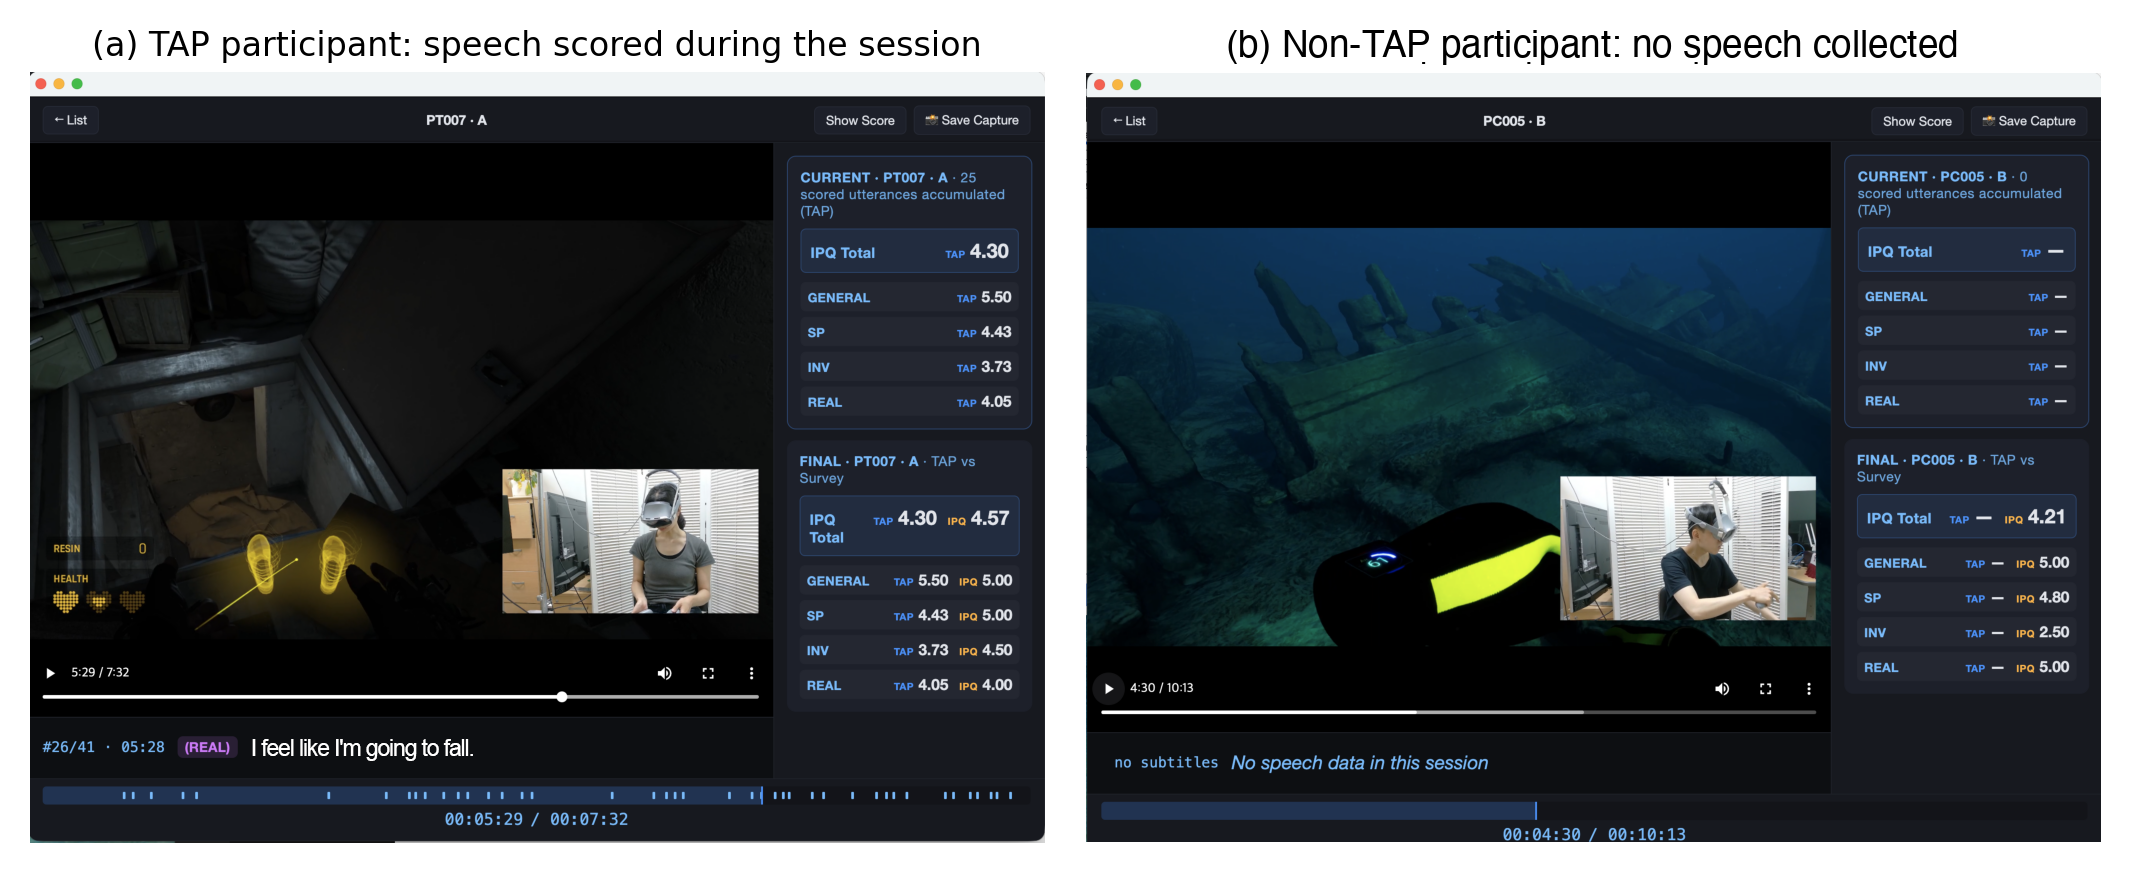
\includegraphics[width=\textwidth]{Figures/F12_viewer_PT_vs_PC.png}
\caption{The analysis interface on a TAP session (a) and a Non-TAP session (b). 
In (a), the panel shows the game view with the participant's webcam inset, the current utterance with the construct the front end routed it to, the utterance timeline with its construct markers, and the running speech-derived IPQ scores beside the self-reported ones. 
In (b), no speech was collected by design, so the utterance track is empty and every speech-derived field is blank while the questionnaire scores remain.}
\Description{Two screenshots of the review application side by side. The left shows a think-aloud session with a subtitle line, construct markers along a timeline, and speech-derived scores. The right shows a non-TAP session with no subtitles, an empty timeline, and dashes in place of the speech-derived scores.}
\label{fig:interface}
\end{figure*}



\begin{figure*}[t]
\centering

\includegraphics[width=\textwidth]{Figures/F03_console.png}
\caption{Experimental setup. \textcircled{\scriptsize 1} Play area: the participant's chair in front of the webcam. \textcircled{\scriptsize 2} Operator console (bottom) and gate monitor with running per-category utterance counts (top). \textcircled{\scriptsize 3} Coverage indicator shown in the headset during the practice session only, hidden in all experimental sessions: four boxes naming the IPQ constructs with example expressions. \textcircled{\scriptsize 4} Real-time transcription window: each recognized utterance with the category assigned by the local front-end classifier and the accumulated cost; from here the operator releases the session to the post-session scoring workflow. \note{korean language needs to be changed}}
\Description{Four panels side by side: a photograph of a chair in a laboratory; a dark operator console with a gate monitor showing five category counters; a virtual reality view with four labeled text boxes for General Presence, Spatial Presence, Involvement, and Experienced Realism; and a transcription log listing Korean utterances with category tags.}
\label{fig:console}
\end{figure*}




% [MCd 2026-09-11] 제목의 "and Refinement" 제거. 리뷰 앱은 점수 편집 기능이 없음 (apps/review-app: 통합기록 xlsx 점수를 읽어 표시만 함). 교수님 문면의 "manually revise the assigned score" 는 2765111 원문 오타 "it does make, alter or adjust the scores" (not 누락) 를 그대로 읽은 결과임. 논문 점수는 전부 파이프라인 산출 그대로.

% The diagram layout was drafted with Gemini image generation from the authors' written specification and redrawn by the authors; every utterance, cue count, score, and aggregate shown is taken from the deployed pipeline's logs.




% An analysis module, developed for post-hoc inspection, aligns and presents each rated item with the utterance that produced its evidence and with the corresponding time-stamped playback of the VR session 
% (see Figure~\ref{fig:interface}). 
% This module is used only for auditing and vignette construction (see Section~\ref{subsec:vignettes}); it does
% [MCd 2026-09-11] 아래 원문 줄은 "it does NOT make, alter or adjust the scores" 의 오타 (not 누락). 교수님 "manually revise" 문장의 출처. 본문은 ②로 정정됨.
% make, alter or adjust the scores.
% Because every rated item carries the timestamp of the utterance that supplied its evidence, it replays how a session score was reached (Section~\ref{subsec:rq1_within}). Figure~\ref{fig:interface} shows the interface at one moment of a think-aloud session (a) and of a control session (b).
\section{EXPERIMENT}
\label{sec:exp}

\subsection{Experimental Design}
\label{subsec:design}

% The study used a \redout{mixed design.}
% \hsnote{The study design followed between-subject study.}
% The protocol was manipulated between participants: the ``TAP'' group thought aloud while playing, whereas the ``non-TAP'' group (as Control) played the same content without a think-aloud process and then completed the same questionnaires. 
% The game was varied within participants: each of the 32 participants (16 per group) played all three titles, yielding 96 sessions.


\hsnote{The study employed a 1 $\times$ 2 between-subjects design with two protocol conditions: TAP and non-TAP (Control). Participants in the TAP group verbalized their ongoing thoughts while playing and completed the post-experience questionnaires after each VR session. Participants in the non-TAP (Control) group experienced the same VR content without concurrent verbalization and completed the same questionnaires after each session. Each participant experienced all three VR games, with the presentation order counterbalanced across participants to minimize potential order effects.}



% Presentation order followed a $3\times3$ Latin square (A--B--C, B--C--A, C--A--B). Orders were not concentrated in either group ($\chi^2$ $p=.913$; TAP 5/6/5, control 6/5/5), and each title occupied each serial position 10--11 times.






\subsection{Experimental Materials}
\label{subsec:material}

\subsubsection{VR Games as Stimuli}


Three commercial VR titles were used: (1) \textit{Half-Life: Alyx}\footnote{Steam: \url{https://store.steampowered.com/app/546560/HalfLife_Alyx/}}, (2) \textit{Subside}\footnote{Steam: \url{https://store.steampowered.com/app/2550040/Subside/}}, and (3) \textit{The Lab}\footnote{Steam: \url{https://store.steampowered.com/app/450390/The_Lab/}}.
\textit{Alyx} and \textit{Subside} were selected to provide highly immersive VR experiences with relatively realistic visual environments, while differing in their interaction and task demands. 
\textit{Alyx} required active, goal-directed interaction, including learning and applying VR-specific mechanics such as the gravity gloves to manipulate objects and progress through the environment. 
In contrast, the selected \textit{Subside} experience primarily involved free underwater exploration with minimal explicit task demands, allowing participants to focus more on observing and navigating the environment. 
\textit{The Lab}'s \textit{Longbow} provided a further contrast as a more stylized and task-oriented experience, in which participants defended a castle by shooting arrows at enemies approaching from multiple directions. 
These VR contents provided variation in visual realism as well as the level and type of interaction required from the participant.



For the TAP practice session, participants experienced \textit{The Lab}'s \textit{Vesper Peak}, a low-demand scene in which they could explore a mountaintop environment and interact with a robot dog by throwing a stick. Its relatively simple interaction was intended to allow participants to focus on practicing the think-aloud procedure before the experiment.

% The practice content for VR setup with think-aloud procedure employed \textit{The Lab}'s Vesper Peak scene, in which the player walks around a mountaintop and throws a stick to a robot dog; the scene demands little of the player, so participants could concentrate and practice on the think-aloud procedure.

\subsubsection{{Apparatus and Physical Setup}}

Experimental sessions ran on a Windows PC (AMD Ryzen 7 7700X, 128\,GB RAM, NVIDIA GeForce RTX 4080) with SteamVR as the active OpenXR runtime. The headset was a Samsung Galaxy XR ($3{,}552 \times 3{,}840$ pixels per eye, $109^{\circ}$ field of view, up to 90\,Hz), streamed from the PC over Wi-Fi through Virtual Desktop; its microphone was the speech input.
Given that immersive system characteristics can support the formation of presence, this high-performance VR setup was selected to provide a high-fidelity and immersive baseline.

The experiment took place in a university laboratory with only the participant and the researcher present. Participants sat in front of a webcam (Figure~\ref{fig:console}~\textcircled{\scriptsize 1}) while playing; the researcher operated the console from an adjacent desk and monitored the procedure and data collection throughout each session.


\subsubsection{Experimental Console}

\hsnote{The experimental console was developed using the Unity 3D game engine to manage experimental sessions and synchronize data collection (Figure~\ref{fig:console}~\textcircled{\scriptsize 2}). At the start of each session, the assigned VR game was launched simultaneously with recordings of the participant's headset view and webcam, as well as real-time speech transcription. All data streams were stored in a session-specific folder using a common timestamp referenced to the session start, enabling temporal alignment across modalities.
During the session, the transcription interface (Figure~\ref{fig:console}~\textcircled{\scriptsize 4}) displayed each recognized utterance together with the category assigned by the front-end classifier, while the console provided session-level monitoring information. After the session, the analysis interface (Figure~\ref{fig:interface}) allowed the recorded utterances to be replayed alongside the participant's corresponding in-game behavior for synchronized review. The collected session data were then passed to the post-session scoring pipeline.}

% A purpose-built Unity application served as the operator console (Figure~\ref{fig:console}~\textcircled{\scriptsize 2}). Starting a session launched the assigned title and, at the same moment, recording of the participant's headset view and webcam and real-time speech transcription, all written to one per-participant, per-game folder on a common time base (milliseconds from session start). The analysis interface (Figure~\ref{fig:interface}) could therefore replay what a participant said alongside what they were doing at that moment. During a session a transcription window (Figure~\ref{fig:console}~\textcircled{\scriptsize 4}) listed each recognized utterance with the category the front-end classifier assigned; from it the operator checked the accumulated cost and released the session to the offline scoring workflow.


\subsubsection{Speech Processing Pipeline}

% For the TAP group, each transcribed utterance was routed by the front-end classifier and scored offline by the multi-agent chain described in Section~\ref{sec:system}; items without evidence were left missing. A coverage indicator (Figure~\ref{fig:console}~\textcircled{\scriptsize 3} Coverage indicator (practice session only): four boxes naming the IPQ constructs with example expressions. 


For the TAP group, each transcribed utterance was routed by the on-device front-end classifier and, after the session, scored by the multi-agent chain described in Section~\ref{sec:system}, whose drafter, reviewer, and rater are API-hosted large language models; only the front end runs on the local machine.
The classifier mapped each utterance to the relevant IPQ dimension, after which the scoring stage determined whether sufficient evidence was available to assign an IPQ item score. Items for which no supporting evidence was identified were retained as missing values rather than imputed. During the practice session only, a coverage indicator (Figure~\ref{fig:console}~\textcircled{\scriptsize 3}) displayed the four IPQ dimensions together with representative expressions to support familiarization with the think-aloud procedure.


For the non-TAP group, transcription, classification, and utterance-based scoring were not run, as these participants received no think-aloud instruction.

% For the control group the classifier was disabled, no practice session was run, and no scoring was performed, since no speech was collected by design.

% \subsubsection{Physical Setup}

% Sessions took place in a university laboratory with only the researcher present. The participant sat in a chair in front of the webcam (Figure~\ref{fig:console}~\textcircled{\scriptsize 1}) and played freely, and the researcher operated the console from a desk beside the play area.






% , administered after every session on its 0--6 scale. The IPQ was chosen over longer instruments because the speech-derived measure needs item-specific evidence for every item, so the item count sets the number of targets the speech must cover.


% , as well as the overall presence score.


% Because concurrent verbalization, i.e., TAP, could add to the demands of playing, workload was measured after each session with the raw NASA Task Load Index (TLX)~\cite{hart1988development,hart2006nasa}, so that any difference in presence between the groups could be read against the load the protocol itself imposed. 
% The six items were averaged with equal weights, since the administered form had no pairwise-comparison items; the form used a 0--10 scale, and scores are reported on the conventional 0--100 metric (form value $\times 10$). The performance item was oriented in the standard direction and was not reversed. 


% \subsubsection{Subjective Measures}
\subsection{Subjective Measures}
\label{subsec:measures}

To address the research questions and hypotheses, subjective measures were selected to evaluate both the validity of the proposed presence measurement approach and the potential influence of the TAP itself. Presence was therefore assessed as the primary outcome, while workload was additionally measured to examine whether concurrent verbalization imposed extra task demands.


Presence was measured with the 14-item Igroup Presence Questionnaire (IPQ)~\cite{schubert2001experience}.
The IPQ was administered after each VR session using a 0--6 scale and assessed General Presence (GP), Spatial Presence (SP), Involvement (INV), and Experienced Realism (REAL).
An overall presence score was calculated as the mean of all 14 items after reverse-scoring SP2, INV3, and REAL1.



Because concurrent verbalization, i.e., TAP, could add to the demands of playing, workload was measured after each session using the NASA Task Load Index (NASA-TLX)~\cite{hart1988development,hart2006nasa}, allowing any differences in presence between the groups to be considered alongside the workload introduced by the protocol itself. The six dimensions—Mental Demand, Physical Demand, Temporal Demand, Performance, Effort, and Frustration—were assessed separately using an 11-point scale from 0 to 10 and analyzed individually.
For reporting, each dimension was converted to the conventional 0--100 scale by multiplying the recorded value by 10. 
% The Performance dimension followed the standard response direction and was not reverse-scored.


% \redout{Cybersickness was measured with the Virtual Reality Sickness Questionnaire (VRSQ)~\cite{kim2018vrsq}: nine items rated 0--3 in an oculomotor and a disorientation factor, each expressed as a percentage of its maximum and averaged without weights.}


% \subsubsection{Objective Measures}

% For the TAP group, each session yielded the think-aloud utterance stream, the category assigned to each utterance by the front-end classifier, the number of IPQ items with construct evidence, and the speech-derived IPQ scores at item, subscale, and total level.

\subsection{Experimental Procedures}
\label{subsec:procedure}

% Participants first completed a short online screening survey (safety items, motion-sickness susceptibility, prior VR experience); anyone who answered yes to a safety item was not enrolled. 
% Eligible respondents were placed in a stratum and assigned to whichever group had fewer participants in it, with one of the three presentation orders, and then scheduled.


% On the day of the experiment, participants provided informed consent before beginning the study.
% Participants in the TAP group first completed a practice session to become familiar with the VR setup and the think-aloud procedure. During this practice session, the coverage indicator (Figure~\ref{fig:console}~\textcircled{\scriptsize 3}) 
% was displayed to support familiarization with verbalizing their ongoing experiences, but it was not shown during the experimental sessions. 
% \note{Participants in the non-TAP (Control) group proceeded directly to the experimental sessions.}

\hsnote{Participants first completed a short online screening survey assessing safety-related eligibility, motion-sickness susceptibility, and prior VR experience. Respondents who met the eligibility criteria were invited to participate in the experiment.}
\hsnote{On the day of the experiment, participants provided informed consent before beginning the study. Participants in the TAP group first completed a VR practice session to become familiar with the think-aloud procedure while using the headset. During this practice session, the coverage indicator (Figure~\ref{fig:console}~\textcircled{\scriptsize 3}) was displayed to support familiarization with verbalizing their ongoing experiences, but it was not shown during the experimental sessions. Participants in the non-TAP (Control) group received a verbal briefing on the VR games and experimental procedure before proceeding to the experimental sessions.}


\hsnote{Each participant then experienced the three VR games in the counterbalanced order. 
Before each session, the researcher briefly explained the game controls and task. Each game was played for approximately 7--10 minutes. 
During the TAP sessions, participants in the TAP group continuously verbalized their ongoing thoughts and experiences. 
If a participant stopped verbalizing for an extended period, a brief synthesized voice prompt (``Please continue thinking aloud'') was presented as a reminder.
After each game, participants completed the post-experience questionnaires, which took about 5--7 minutes and served as a rest.}



% was visible only in this practice session and never during the experimental sessions. Control participants started directly with the first game. Each game was played for about 7--10 minutes, preceded by a short explanation of how to play; whenever a TAP participant stopped thinking aloud, the researcher triggered a short synthesized voice prompt (``Please continue thinking aloud''). 
% After each game, participants completed the questionnaires, which took 3--5 minutes and served as a \note{10-minute} break before the next game.

\subsection{Participants}
\label{subsec:participants}

% Thirty-two participants (16 female, 16 male; age $M=26.2$ years, $SD=3.1$, range 21--34; no participant chose ``prefer not to disclose'') were included in the analyses, 16 in the TAP group and 16 in the non-TAP (Control) group, each participating in three VR game sessions. 

%\hsnote{Thirty-two participants (16 female, 16 male; age $M=26.2$ years, $SD=3.1$, range 21--34; no participant chose ``prefer not to disclose'') were included in the analyses. 
%Following a between-subjects design, they were divided into two groups of 16: the TAP group and the non-TAP (Control) group. Each participant completed three VR game sessions.}
%They were recruited through advertisements on university online communities and posters on campus and in nearby residential areas; by the stratification variable, half of each group fell in the high prior-VR-experience stratum, and six studied or worked in a VR-related field. 

\hsnote{Thirty-two participants (16 female, 16 male; no participant selected ``prefer not to disclose''; age $M=26.2$ years, $SD=3.1$, range 21--34) were included in the analyses.
Following the between-subjects design, participants were evenly assigned to the TAP and non-TAP (Control) groups, with 16 participants in each group.
Within their respective groups, each participant completed three VR game sessions.}
Participants were recruited through advertisements posted on university online communities, campus bulletin boards, and nearby residential areas.


% Following a between-subjects design, they were divided into two groups of 16: the TAP group and the non-TAP (Control) group. 
% In their respective groups, each participant completed three VR game sessions. 

% \redout{; six studied or worked in a VR-related field.}
% 이거는 밑에 참가자 균형 이야기할 때 포함되어야 함. 

To maintain comparable participant characteristics across the two between-subjects groups, participants were assigned to balance motion-sickness susceptibility, prior VR experience, and gender between the TAP and non-TAP groups. Both groups included 8 female and 8 male participants.

Prior VR experience was characterized using three indicators. First, 14 participants in the TAP group and 13 participants in the non-TAP group had prior VR experience, while 2 and 3 participants, respectively, had no prior experience. Among those with prior VR experience, 12 participants in the TAP group reported a cumulative VR usage time of 10 hours or less and 2 reported more than 10 hours; in the non-TAP group, 9 reported 10 hours or less, and 4 reported more than 10 hours. Regarding recency of VR use, the TAP group included 6 participants who had used VR within the past month, 5 within the past year, and 3 more than one year ago. The corresponding numbers in the non-TAP group were 6, 5, and 2 participants, respectively.
Overall, these distributions indicate that prior VR experience was broadly comparable between the two groups.

Motion-sickness susceptibility was scored from the screening survey's MSSQ items~\cite{golding1998mssq} and did not differ between groups (TAP $M=5.72$, $SD=4.05$; non-TAP $M=6.06$, $SD=4.30$; Welch's $t=-0.23$, $p=.82$) and age was also comparable across groups (TAP: $M=25.8$ years, $SD=2.8$; non-TAP: $M=26.6$ years, $SD=3.4$).


% To maintain comparable participant characteristics across the two groups, assignment was stratified based on motion-sickness susceptibility (high/low) and prior VR experience (high/low). This $2 \times 2$ stratification produced four strata, each filled with four TAP and four non-TAP participants (4 strata $\times$ 4 $\times$ 2 groups $= 32$). Gender was not a stratification variable; assignment aimed at gender balance where the applicant pool allowed, yielding 8~F~/~8~M in each group. The two groups showed no significant difference in motion-sickness susceptibility ($M=5.72$ vs.\ $6.06$; $t=-0.227$, $p=.822$), and age was comparable across groups (TAP: $M=25.8$ years, $SD=2.8$; non-TAP: $M=26.6$ years, $SD=3.4$).

This study was approved by the university's institutional review board (No.\ anonymized for review). 
Participants consented to the recording of the experimental sessions, survey completion, and to the pseudonymized processing of their utterances by the automated scoring pipeline. Each participant received USD 14 for taking part; the whole experiment took about 70 minutes.

% camera-ready: KUIRB-2026-0416-01



%\hsnote{To maintain comparable participant characteristics across the two groups, assignment was stratified based on motion-sickness susceptibility and prior VR experience. Participants with higher and lower levels of each characteristic were distributed evenly between the TAP and non-TAP groups. The two groups showed no significant difference in motion-sickness susceptibility ($M=5.72$ vs.\ $6.06$; $t=-0.227$, $p=.822$).} \note{need other data}


%This study was approved by the university's institutional review board (No. anonymized for review). 
%Participants consented to the recording of the experimental sessions, survey completion, and to the pseudonymized processing of their utterances by the automated scoring pipeline.
%Each participant received \$14 for the session. 
%The entire experiment took about 70 minutes.



% camera-ready: KUIRB-2026-0416-01
\section{RESULTS}
\label{sec:result}

\subsection{Analysis Method}
\label{subsec:analysis}


Because each participant contributed three sessions, session-level records are not independent. Between-group contrasts were computed on participant-level means over the three games ($n=16$ per group) with Welch's $t$-test; within-participant contrasts across games used paired $t$-tests. Convergent validity between speech-derived and self-reported IPQ scores was quantified with Pearson's $r$ and Spearman's $\rho$ at the session level, the participant level, and on within-participant deviation scores (each participant's own mean removed), which isolate variation across games within the same person. Because the pipeline's final anchoring and aggregation rules were selected on the first seven participants (21 sessions) using agreement with self-report as one criterion, those participants form a development sample; the remaining nine (27 sessions) were scored after the pipeline was frozen and serve as a held-out confirmation sample. The primary convergence estimate is reported on the held-out sample with participant-clustered bootstrap confidence intervals (5{,}000 resamples of participants); the development sample and the pooled 48 sessions are reported alongside.

The primary evaluation unit for the speech-derived IPQ is the total score, following the IPQ reporting guideline~\cite{tran2024ipq} and our own coverage findings: INV is the least covered subscale and its within-participant correlation is null (Sections~\ref{subsec:sample} and~\ref{subsec:rq1_convergence}). Subscale results are complementary, not parallel primary indicators. Within-person agreement for the total (Section~\ref{subsec:rq1_within}) was assessed against a chance baseline from randomly re-assigning the speech-derived scores across the same participant's three games ($20{,}000$ permutations); binomial $p$ values are reported for comparison and yield the same conclusions.

Familywise error across the five group-comparison measures was controlled with the Holm--Bonferroni procedure; uncorrected and corrected $p$ values are both reported, and asterisks in tables mark uncorrected $p<.05$ only. Effect sizes are Cohen's $d$, with Hedges' $g$ and its 95\% CI for the primary group contrast; classification recall carries Wilson 95\% CIs. Missing values were left missing, and the significance level was 5\%.

Because a non-significant level difference is not evidence of agreement, the level comparison between speech-derived and self-reported totals was complemented with equivalence testing (TOST~\cite{lakens2017equivalence,lakens2018tutorial}), as used earlier in VR measurement studies~\cite{lee2012equivalence,sanaei2024scene,johnsdorf2025memory}. No consensus margin exists for the IPQ, so the primary margin was the smallest detectable change derived from the questionnaire's own $SEM$ ($\alpha=.87$~\cite{schwind2019presence} in VR settings; $SD$ from the full 32-participant sample), with sensitivity analyses under three alternative rules ($1.96\,SEM$, own-sample $\alpha$, TAP-only $SD$). Equivalence tests were run at the participant level ($n=16$). Individual-level agreement was quantified with Bland--Altman limits of agreement~\cite{bland1986statistical} and Lin's concordance correlation~\cite{lin1989concordance}, because equivalence of means does not imply interchangeability of individual scores.

An INV-side calibration term ($+0.5535$, the observed INV level offset) is reported alongside the uncorrected numbers in Section~\ref{subsec:rq1_convergence}; it is not applied to the primary indicator, and the direction and rank analyses use the uncalibrated indicator throughout.


\subsection{Sample and Data Coverage}
\label{subsec:sample}

Self-reported IPQ scores were available for all 96 sessions. Speech-derived IPQ scores exist only for the TAP group, where the pipeline produced a primary-indicator score for all 48 sessions from a total of 3{,}595 utterances (\textit{M} $=74.90$ utterances per session, \textit{SD} $=25.33$). The non-TAP group produced no think-aloud data by design, so all speech-based analyses below are restricted to the TAP group.

Coverage was uneven at the item level (Figure~\ref{fig:missing_items}). Across the 48 TAP sessions, a mean of 9.54 of the 14 IPQ items ($SD=2.00$, $Mdn=10$, range 5--13) carried at least one piece of supporting evidence; no session had all 14 items covered, and five sessions covered fewer than seven. Item-level gaps were concentrated in the involvement subscale: INV1 was uncovered in 46 of 48 sessions (95.8\%), INV3 in 43 (89.6\%), and INV2 in 31 (64.6\%), followed by REAL4 in 26 (54.2\%). The remaining ten items were uncovered in 14 or fewer sessions each. In total, 214 item slots were uncovered, a mean of 4.46 per session.

\paragraph{Reliability of the reference instrument.}
The self-reported IPQ served as the reference against which the speech-derived score is evaluated, so its own reliability bounds how closely any second measure can be expected to track it. Computed on participant-level item means over the three games ($n=32$), Cronbach's $\alpha$ for the 14-item total was $.816$, in the range reported for the IPQ in VR studies ($\alpha=.87$~\cite{schwind2019presence}); the subscales were less consistent (SP $.741$, INV $.714$, REAL $.684$; GP is a single item). Corrected item--total correlations ranged from $.129$ (INV1) to $.776$ (INV4); INV1, the item least covered by speech (Section~\ref{subsec:sample}), was also the item most weakly bound to the questionnaire total. Reliability differed by group in one subscale: the SP subscale was consistent in the non-TAP group ($\alpha=.869$) but not in the TAP group ($\alpha=.191$), while the totals were comparable (non-TAP $.829$, TAP $.700$). With 16 participants per group this contrast is fragile, and we treat it as a hypothesis about the protocol's effect on spatial-presence self-report, not as a finding (Section~\ref{subsec:rq3}).


\begin{figure}[t]
\centering
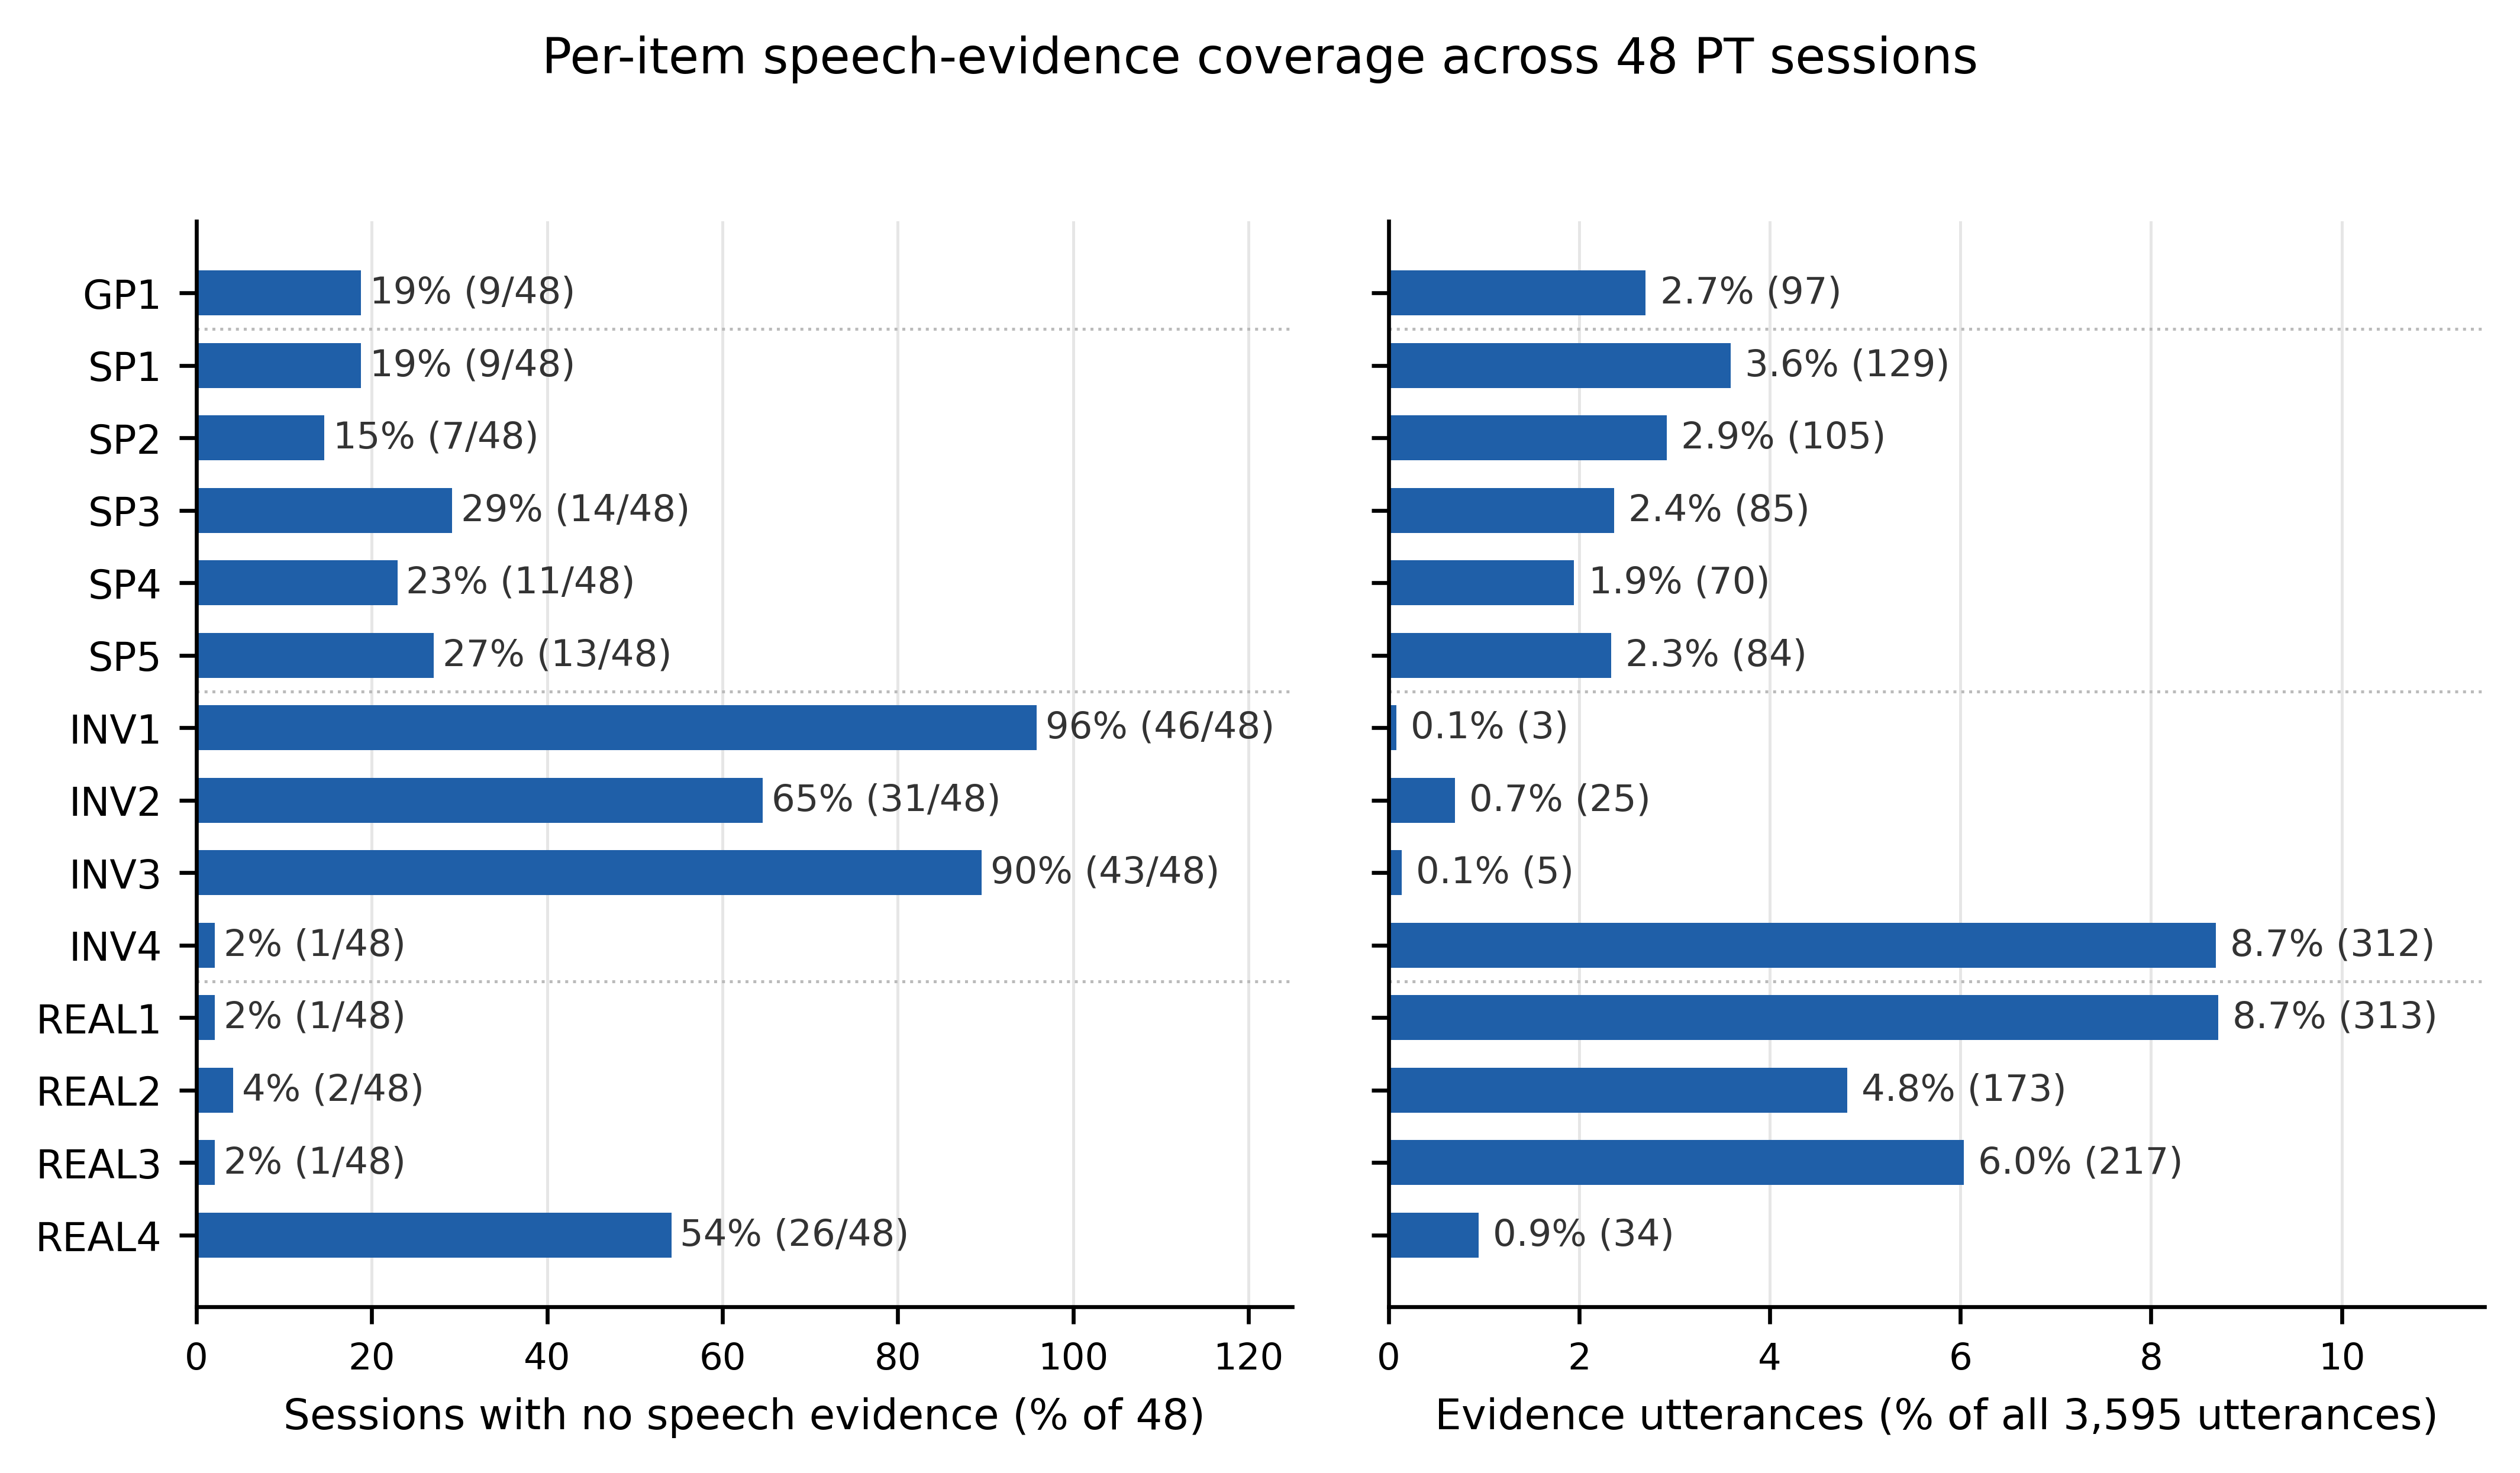
\includegraphics[width=0.85\linewidth]{Figures/F04b_item_coverage.png}
\caption{Per-item speech-evidence coverage across the 48 TAP sessions. Left: share of sessions in which the item received no speech evidence. Right: evidence utterances per item as a share of all 3{,}595 utterances (counts in parentheses; an utterance can support more than one item, so shares do not sum to 100\%). INV1 and INV3 were supported by 3 and 5 utterances in total, whereas INV4 and REAL1 each drew over 300.}
\label{fig:missing_items}
\Description{Bar chart of uncovered-session counts per IPQ item, with INV1, INV3, and INV2 leading.}
\end{figure}


\subsection{RQ1a: Within-Person Agreement in Presence Direction Across VR Games}
\label{subsec:rq1_within}

The primary RQ1 test is the held-out convergence reported in Section~\ref{subsec:rq1_convergence}; this section reports the secondary within-person indicators, which ask whether the speech-derived IPQ total tracks the direction of a participant's own presence differences across the three VR games. Table~\ref{tab:within_person} reports three within-person agreement rates against their chance baselines, with permutation and binomial $p$ values.

Within a participant, the speech-derived total picked the participant's own highest-presence game (top-1) in $11$ of $16$ cases (\textbf{69\%}) against a chance baseline of $33\%$. Considering the three ordered pairs a participant contributes (with ties on the questionnaire excluded), the speech-derived total agreed with the survey on the direction of $35$ of $46$ pairs (\textbf{76\%}) against a chance baseline of $50\%$. The complete three-game rank matched in $5$ of $16$ cases ($31\%$), above the chance baseline of $17\%$ but not statistically distinguishable from chance at the current sample size. The mean per-participant Spearman correlation between speech and survey rankings across the three games was $\rho=0.59$. Figure~\ref{fig:within_participant_profiles} shows each participant's three-game profile under both measures.

\begin{table}[t]
\centering
\caption{Within-participant agreement between speech-derived and self-reported IPQ total across the three VR games ($n=16$). Chance baselines assume random re-assignment of the speech scores among the same participant's three games. The permutation test re-assigns speech scores across the same participant's three games ($20{,}000$ permutations) and is the primary reference; the binomial test is included for comparison.}
\label{tab:within_person}
\small
\begin{tabular}{lcccc}
\hline
Indicator & Observed & Chance & $p_{\mathrm{perm}}$ & $p_{\mathrm{binom}}$ \\
\hline
Top-1 game match & $11/16 = 69\%$ & $33\%$ & $.0037$ & $.0040$ \\
Pairwise direction match & $35/46 = 76\%$ & $50\%$ & $.0006$ & $.0003$ \\
Complete 3-game rank match & $5/16 = 31\%$ & $17\%$ & n/a & $.1134$ \\
Mean per-participant Spearman $\rho$ & $0.59$ & $0$ & --- & --- \\
\hline
\end{tabular}
\end{table}

Table~\ref{tab:within_by_construct} in Appendix~\ref{sec:appendix} shows the same within-person indicators computed on the four subscales. INV shows a within-person top-1 rate of $73\%$ that comes with a null within-person correlation (Section~\ref{subsec:rq1_convergence}), consistent with the interpretation that the subscale rank is dominated by a few sessions in which any INV evidence was found at all; the total score is the more robust indicator on the current sample.


Two observations on the direction indicators of the total. First, when the pipeline missed the top-1 game (5 of 16 cases), the disagreement was concentrated on a single game contrast: in every one of the five cases the questionnaire's top game was Alyx and the pipeline's top game was Subside; Subside was the pipeline's top game for $12$ of $16$ participants and the questionnaire's top game for $8$ of $16$. Second, The Lab was near-uniformly the lowest-presence game (questionnaire $13/16$, pipeline $11/16$), so most of the within-person signal lives in the Alyx--Subside contrast.

Between-participant rank agreement was smaller than within-participant agreement: ranking the sixteen participants by their three-game mean, the Spearman correlation between speech-derived and self-reported ranks was $\rho=0.49$. We therefore read the total-score result primarily at the within-person level.


\begin{figure*}[t]
\centering
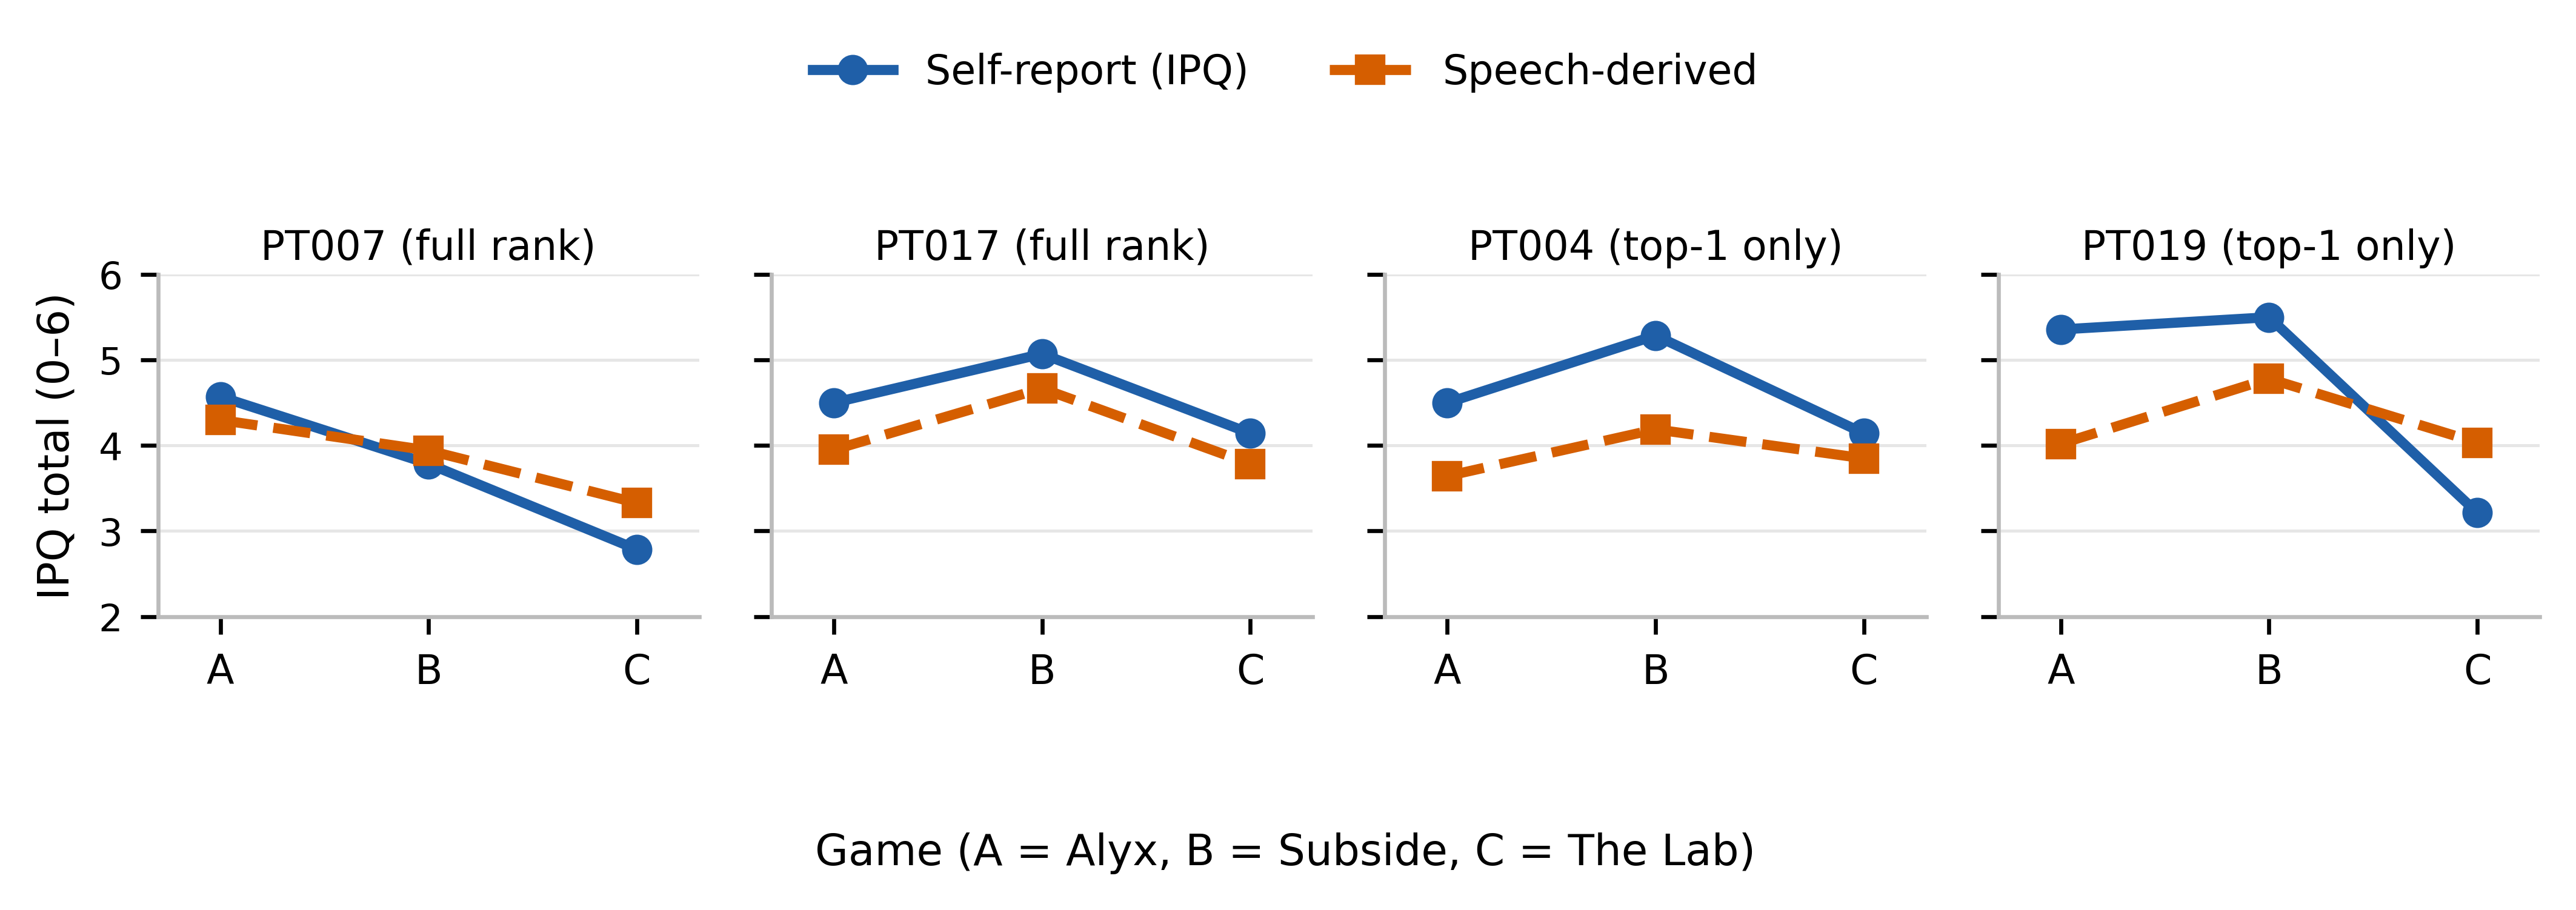
\includegraphics[width=\textwidth]{Figures/F11_within_participant_profiles.png}
\caption{Within-participant three-game profiles of the IPQ total for four participants, selected as two whose three-game rank the speech score reproduced in full and two for which only the highest-presence game matched. Within each panel the three VR games sit on the horizontal axis and the IPQ total ($0$--$6$) on the vertical axis; the self-reported score is a solid line with circular markers and the speech-derived score a dashed line with square markers. Across all 16 participants the speech-derived total matched the direction of $35/46 = 76\%$ of ordered game pairs (permutation $p=.0006$), picked the participant's own highest-presence game in $11/16 = 69\%$ of cases (permutation $p=.004$), and reproduced the complete three-game rank in $5/16 = 31\%$ of cases (n.s.).}
\label{fig:within_participant_profiles}
\Description{Four per-participant panels in one row showing speech-derived and self-reported IPQ totals across the three VR games, with panel titles indicating full rank or top-1 only.}
\end{figure*}


Because every rated item carries the timestamp of the utterance that supplied its evidence, the interface also replays how a session score was reached. Figure~\ref{fig:trajectory} shows the same four participants' sessions as they accumulated. Recomputing from the complete evidence returns the reported session score for 240 of 240 session-by-index values across the 48 sessions (agreement within $0.002$), so the replay and the reported score are one quantity read at different times; across those sessions the total moved a median of $1.01$ points over a whole session and $0.24$ points over its second half.

\begin{figure*}[t]
\centering
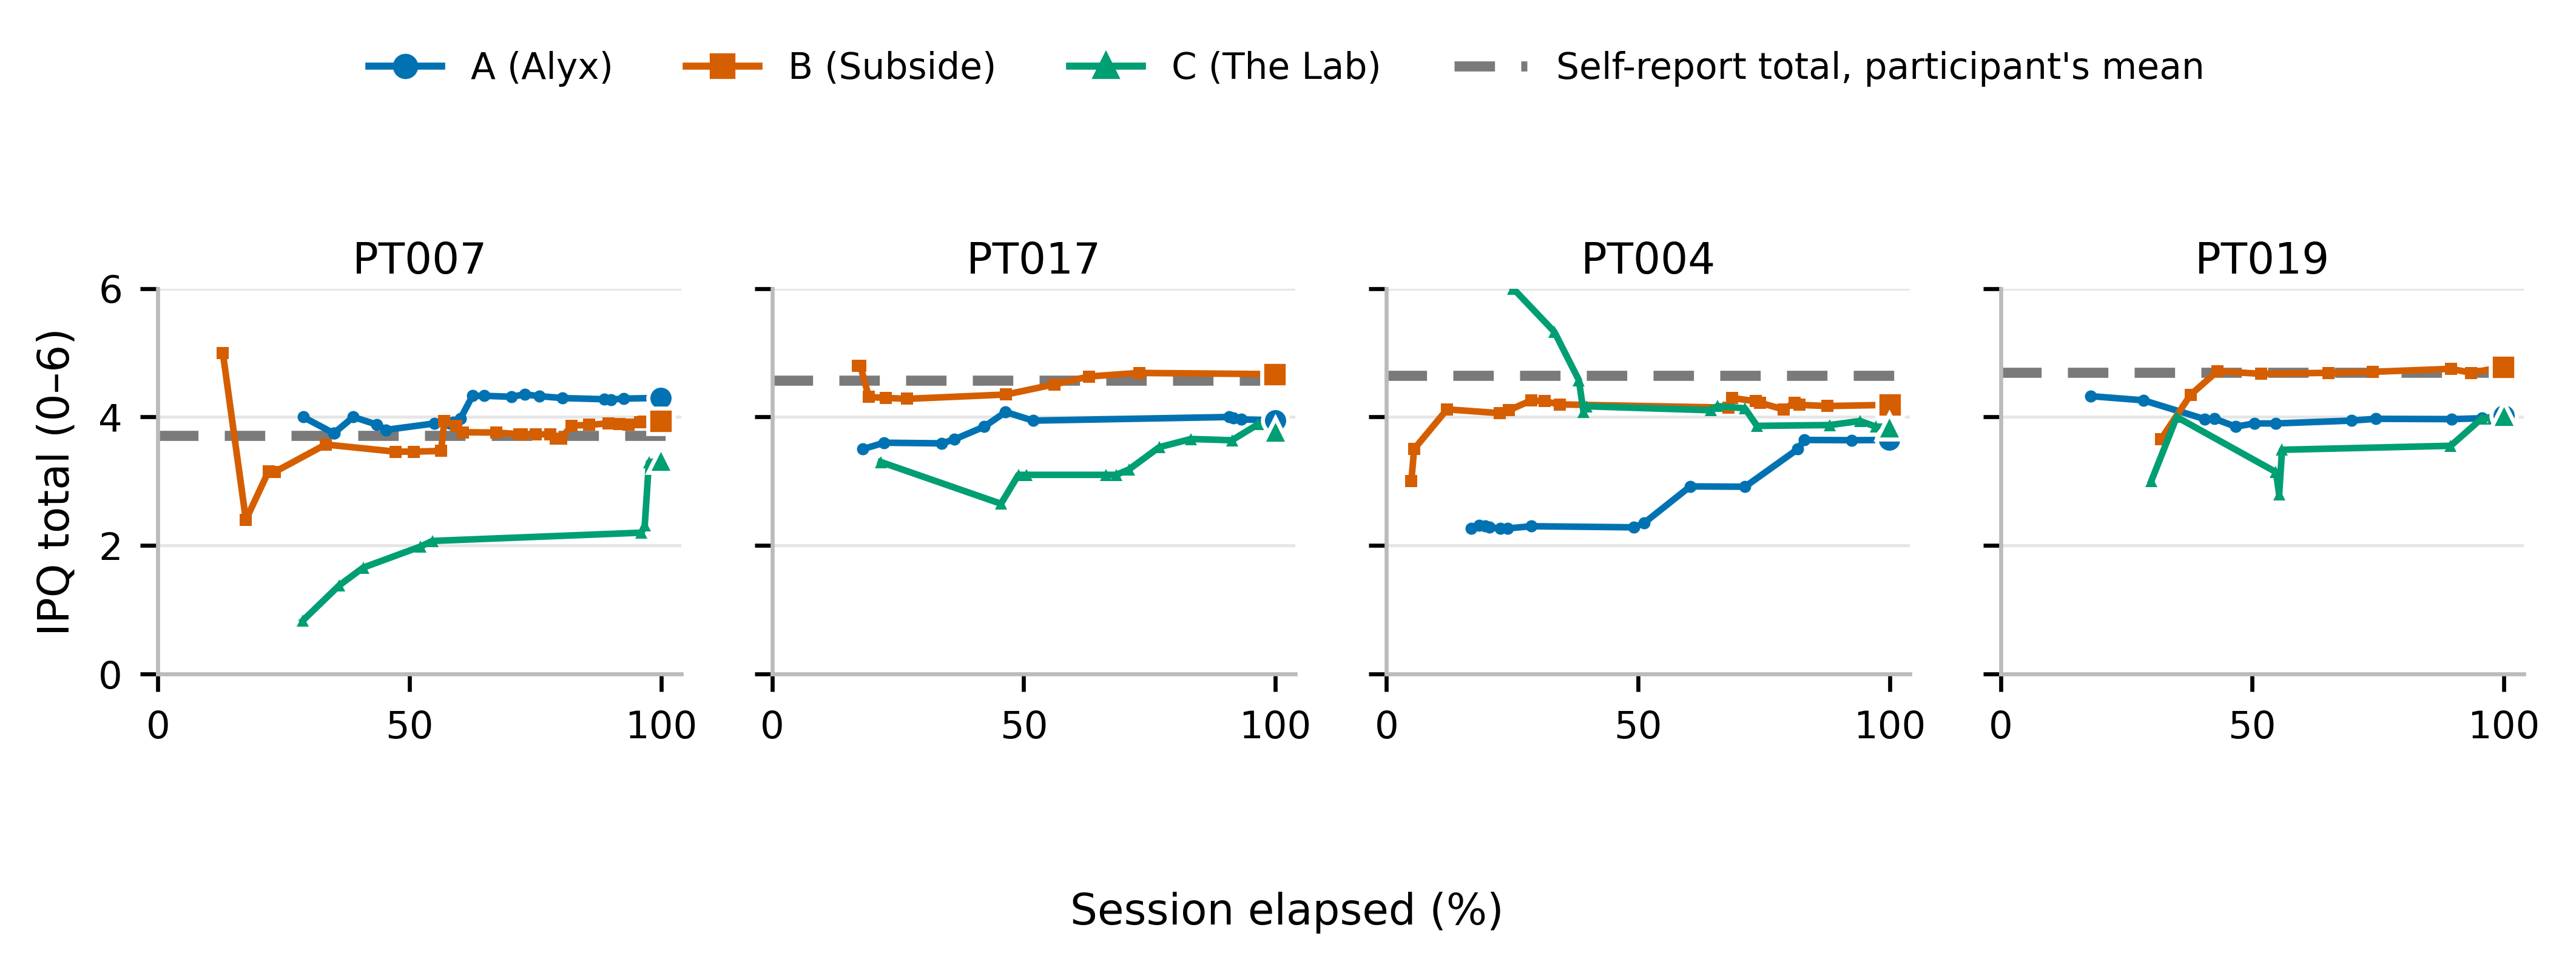
\includegraphics[width=\textwidth]{Figures/F13_score_trajectory.png}
\caption{Speech-derived IPQ total accumulating through each session, shown for four participants with one line per VR game. Each point recomputes the evidence-gated score from all item evidence available up to that moment, using the aggregation applied to the session score. The filled marker ending each line is the session score reported in the results. The grey dashed line is the participant's mean self-reported total across the three sessions, shown as a single reference; the per-game comparison of speech-derived and self-reported scores is given in Figure~\ref{fig:within_participant_profiles}. Sessions carried a median of 14 evidence utterances (range 8 to 55), so the earliest points rest on one or two items.}
\Description{Four small panels side by side, one per participant. Each panel plots three cumulative score lines, one per VR game, against percentage of session time elapsed, with filled end markers and a single grey dashed reference line.}
\label{fig:trajectory}
\end{figure*}

\subsection{RQ1b: Convergence and Level Offset}
\label{subsec:rq1_convergence}

On the held-out confirmation sample (9 participants, 27 sessions), the speech-derived IPQ total correlated moderately to strongly with the self-reported total ($r=+.608$, $p=.0008$; participant-clustered bootstrap 95\% CI $[+.26, +.85]$; $\rho=+.615$, $p=.0006$). The association held at the participant level (three-session means, $r=+.818$, $n=9$, $p=.007$) and within participants after removing individual means ($r=+.469$, $p=.014$). Session-level intraclass correlation of the questionnaire total was low ($\mathrm{ICC}=.09$), so the 27 sessions correspond to roughly 23 effectively independent observations. The development sample, on which the pipeline had been selected, showed a weaker and non-significant association ($r=+.285$, $p=.21$, $n=21$), and the pooled 48 sessions fell between the two ($r=+.419$, $p=.003$; clustered CI $[+.20, +.67]$). Applying the INV calibration constant Applying the INV calibration constant (Table~\ref{tab:calibration_prepost} in Appendix~\ref{sec:appendix}) left the held-out correlation significant but lower ($r=+.525$, $p=.006$); because that constant was estimated on all 47 scored sessions, uncalibrated scores are reported as primary.

\begin{table}[t]
\centering
\caption{Held-out, development, and pooled convergence of the speech-derived IPQ total with the self-report, on the same 16 TAP participants split by whether they were used to select the pipeline.}
\label{tab:heldout_convergence}
\small
\begin{tabular}{lcccccc}
\hline
Sample & Participants & Sessions & $r$ & $p$ & Clustered 95\% CI & $\rho$ \\
\hline
Held-out & 9 & 27 & $+.608$ & $.0008$ & $[+.26,\ +.85]$ & $+.615$ \\
Development & 7 & 21 & $+.285$ & $.21$ & --- & --- \\
Pooled & 16 & 48 & $+.419$ & $.003$ & $[+.20,\ +.67]$ & --- \\
\hline
\end{tabular}
\end{table}

For reference, Table~\ref{tab:convergence} in Appendix~\ref{sec:appendix} reports the correlation between the speech-derived IPQ score and the self-reported IPQ score at the three levels of aggregation on the pooled sample (16 participants, 48 sessions). At the session level the total score converged at $r=+.419$ ($p=.003$), and the rank-based estimate was of comparable size ($\rho=+.461$, $p=.001$). Aggregating to participant means raised the point estimate but widened the interval implied by the smaller sample ($r=+.488$, $p=.055$, $n=16$). The within-participant estimate, which asks whether a participant's speech scores rise and fall across games in step with that participant's own questionnaire responses, was $r=+.386$ ($p=.007$).

The subscales diverged sharply. On the within-participant estimate, REAL ($r=+.418$, $p=.003$), GP ($r=+.416$, $p=.009$), and SP ($r=+.293$, $p=.046$) all showed positive convergence, whereas INV was effectively zero and slightly negative ($r=-.055$, $p=.715$). Per-construct, per-level correlations with their confidence intervals are given in Table~\ref{tab:convergence}.


Convergence in rank order was accompanied by a systematic offset in level. Comparing the two scores within the same session (Table~\ref{tab:levelbias}, Figure~\ref{fig:bland_altman}), the speech-derived total score sat below the self-reported total by $-0.232$ points on the $0$--$6$ scale ($t(47)=-2.286$, $p=.027$, $d=-0.330$). The offset was largest for INV ($-0.554$, $p=.003$, $d=-0.456$) and present for SP ($-0.245$, $p=.041$), while GP ($+0.010$, $p=.940$) and REAL ($-0.005$, $p=.975$) showed no offset.

\begin{table}[t]
\centering
\caption{Level offset between the speech-derived and self-reported IPQ scores within the same session (speech $-$ survey), TAP group. Asterisks mark uncorrected $p<.05$.}
\label{tab:levelbias}
\small
\begin{tabular}{lccccc}
\hline
Scale & $n$ & $M$ diff & $SD$ & $t$ & $p$ \\
\hline
Total & 48 & $-0.232$ & $0.703$ & $-2.286$ & $.027$* \\
GP & 39 & $+0.010$ & $0.845$ & $+0.076$ & $.940$ \\
SP & 47 & $-0.245$ & $0.799$ & $-2.098$ & $.041$* \\
INV & 47 & $-0.554$ & $1.213$ & $-3.128$ & $.003$* \\
REAL & 48 & $-0.005$ & $1.101$ & $-0.031$ & $.975$ \\
\hline
\end{tabular}
\end{table}

\begin{figure*}[t]
\centering
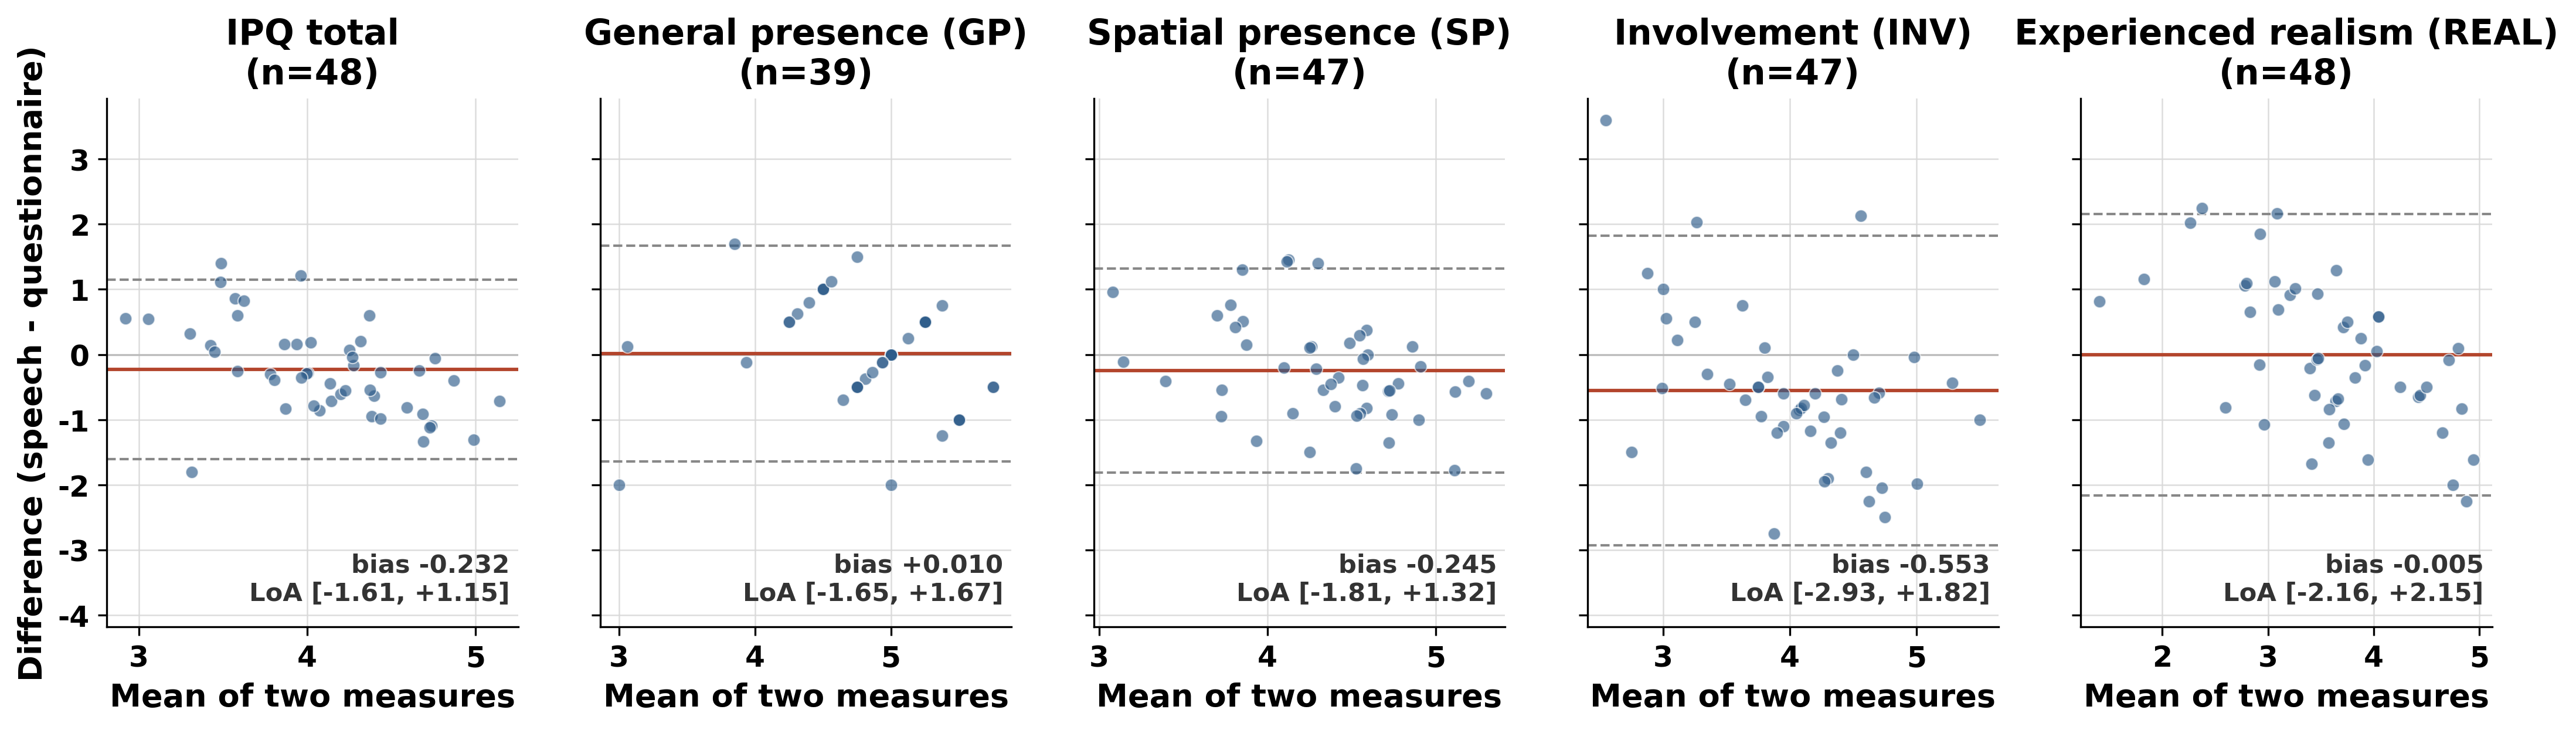
\includegraphics[width=\linewidth]{Figures/G02_bland_altman.png}
\caption{Bland--Altman plot of speech-derived vs.\ self-reported IPQ scores by construct. Mean bias and 95\% limits of agreement are drawn per construct.}
\label{fig:bland_altman}
\Description{Bland-Altman scatter with per-construct bias lines and agreement bands.}
\end{figure*}

\paragraph{Equivalence within the measurement error of the questionnaire.}
The level offset, although statistically detectable, was smaller than the measurement error of the reference instrument. At the participant level the speech-derived total sat $-0.232$ points below the questionnaire total ($SE=0.095$, $n=16$, paired $t$ $p=.028$), whereas the questionnaire's own standard error of measurement, from $\alpha=.87$~\cite{schwind2019presence} and the between-participant $SD$ of $0.579$ in the 32-participant sample, was $SEM=0.209$, giving a smallest detectable change of $SDC=0.579$. Against this margin the two totals were statistically equivalent (TOST $p=.001$), and equivalence also held under the stricter $1.96\,SEM$ margin of $\pm0.409$ ($p=.041$), under our own-sample $\alpha$ of $.816$ ($\pm0.486$, $p=.009$; $\pm0.688$, $p<.001$), and under the SDC computed from the TAP-only $SD$ ($\pm0.426$, $p=.029$). The one combination that failed was the strictest, TAP-only $SD$ with the $1.96\,SEM$ rule ($\pm0.302$, $p=.237$); Table~\ref{tab:equivalence} lists all combinations. An item-level mixed model with crossed random effects for participant and item, which accommodates the participant-specific pattern of missing items directly, estimated the method effect at $-0.297$ (90\% CI $[-0.411, -0.183]$; 458 item pairs), inside the SDC margin and touching the $1.96\,SEM$ bound. Equivalence held for every subscale under the same rules (SP $p=.002$, INV $p=.027$, REAL $p<.001$ at $1.96\,SEM$), but the subscale margins are wide because subscale reliability is lower, so we do not treat the subscale results as independent evidence.

Equivalence of means did not extend to interchangeability of individual scores. The 95\% limits of agreement for sessions were $[-1.609, +1.146]$, wider than the questionnaire's SDC, and Lin's concordance correlation was $.339$ at the session level and $.368$ at the participant level. Read against the percentile norms compiled from two decades of IPQ studies~\cite{tran2024ipq}, the group means fell in adjacent classes (questionnaire $1.20$, ``Very High''; speech $0.97$, ``High'' on the $-3$ to $+3$ metric); four of the 16 participants were classified identically by the two measures and 14 within one class, and in 11 of the 12 mismatches the speech-derived class was the lower one.

Applying the INV-side calibration term ($+0.5535$) to INV item scores and re-aggregating changes the level indicators of the total while leaving the within-person direction indicators of the total essentially unchanged (Table~\ref{tab:calibration_prepost} and Figure~\ref{fig:calibration_bias}; the participant sample size shrinks from $16$ to $15$ under the calibration input file because one participant is dropped for having fewer than three fully covered games). The mean speech--survey level offset on the total moved from $-0.221$ to $-0.134$ (pre-post reduction $=0.087$; the pre-calibration figure differs from the $-0.232$ reported above because it is computed on these 15 participants), the mean absolute error from $0.603$ to $0.584$, and the fraction of sessions within $\pm0.5$ from $45\%$ to $49\%$; the fraction of sessions with speech below survey moved from $64\%$ to $60\%$. On INV, the offset moved from $-0.554$ to $-0.000$ and the mean absolute error from $1.070$ to $0.845$. As expected for an additive constant applied within participants, the within-participant top-1, pairwise, and complete-rank rates for INV were unchanged by calibration; the top-1 and pairwise rates for the total moved slightly ($67\%\rightarrow60\%$ top-1 on the $n=15$ sub-sample; $77\%\rightarrow72\%$ pairwise). One session crossed the $6.0$ ceiling under calibration. We report both the uncalibrated and the calibrated numbers here, and keep the uncalibrated primary indicator for the direction analyses in Section~\ref{subsec:rq1_within}.

\begin{figure}[t]
\centering
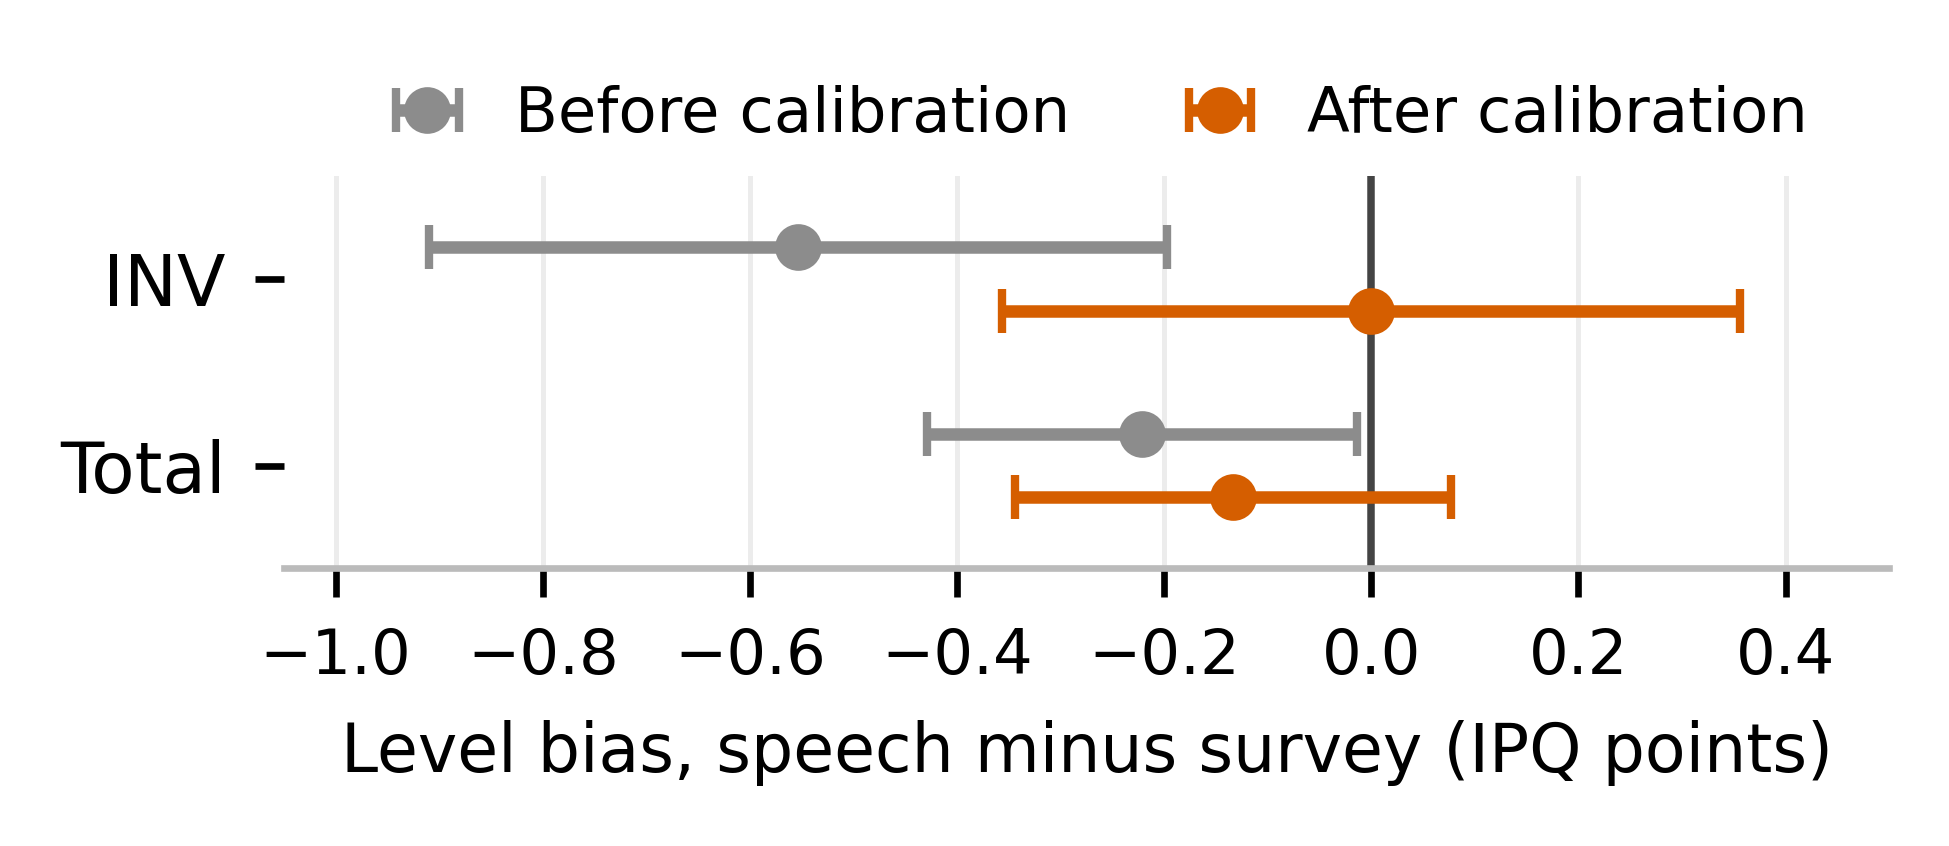
\includegraphics[width=0.5\linewidth]{Figures/F07_calibration_bias.png}
\caption{Level offset (speech minus survey) on the involvement subscale and on the total, before and after the INV-side calibration. Points are means with 95\% confidence intervals over the 47 sessions that carry a calibrated value.}
\label{fig:calibration_bias}
\Description{Horizontal interval plot comparing the mean level offset before and after calibration for the involvement subscale and the total.}
\end{figure}

Neither the amount of speech nor the amount of extracted evidence predicted the resulting score. Within the TAP sessions, the number of utterances was unrelated to the number of evidenced items ($r=+.126$, $p=.394$), to the speech-derived total ($r=+.074$, $p=.619$), and to the self-reported total ($r=+.074$, $p=.618$). The number of evidenced items was likewise unrelated to the speech-derived total ($r=+.180$, $p=.222$) and to the speech--survey level offset ($r=+.043$, $p=.771$).

Restricting the score to items backed by evidence changed almost nothing relative to scoring every item. The primary-indicator total differed from the all-item variant by $+0.018$ on average (mean absolute difference $0.093$, maximum $0.490$); the largest subscale movement was again INV ($-0.046$; mean absolute difference $0.191$, maximum $0.888$), while GP was identical and REAL differed by $+0.007$.


\subsection{Reliability of Speech Scoring (Human-Coder Reference)}
\label{subsec:rq1_reliability}

Automated scoring is judged against the agreement between independent human raters, which bounds what a scorer modeled on human judgment can reach~\cite{williamson2012framework}. To obtain this reference, two coders uninvolved in the pipeline design scored 12 of the 48 TAP sessions (four sessions from the two participants whose speech-derived and self-reported top games disagreed, PT013 and PT001, plus eight game-stratified random draws) from the raw transcripts, blind to video, survey, and pipeline output, under the pipeline's evidence rule: for each of the 14 IPQ items, whether evidence was present and, if so, a 0--6 score. Coders received the item definitions, evidence rule, and worked examples given to the LLM rater but not its norm-referenced intensity bands, so coder--LLM agreement does not reflect a shared intensity calibration.

The two coders agreed on whether evidence was present in 81\% of the 168 item slots (Cohen's $\kappa=.39$) and, where both scored, reached a quadratic weighted $\kappa$ of $.39$ and an ICC(2,1) of $.42$ at the item level. The pipeline's agreement with each coder fell within $.10$ of this human ceiling (QWK $.42$ and $.37$; ICC $.44$ and $.38$), which meets the relative criterion of Williamson et al.~\cite{williamson2012framework} but not their absolute threshold of $.70$, a level the coders themselves did not reach. Treated as a third rater on the 99 slots all three scored, the pipeline deviated least from the other two (mean deviation $-0.46$ vs.\ $+0.99$ and $-0.53$) and left inter-rater ICC unchanged ($.42 \to .42$). At the session level, however, agreement dropped (coder--coder QWK $.28$ vs.\ coder--pipeline $.06$ and $-.02$), a divergence we return to below.

The divergence has two identifiable sources. One is rater level: one coder scored about one point above both the other coder ($+1.01$) and the pipeline ($+0.99$), whereas the other coder and the pipeline agreed on level ($-0.00$), so the apparent human--machine gap is largely one rater's calibration. The other is evidence detection. Across the 168 slots the pipeline found no evidence in 33\%, close to the share in which neither coder did (29\%), but the disagreements were one-sided: 40 slots were evidenced by a coder and missed by the pipeline against one the reverse, concentrated on INV1 (missed in 12 of 12 sessions by the pipeline, 4 by both coders), INV3 (11 vs.\ 2), INV2, and REAL4. Section~\ref{sec:discussion} traces this pattern to the aggregation rule for absence-scored items.

\subsection{RQ2: Front-End Classification and Pipeline Reach}
\label{subsec:rq2}

RQ2 concerns the locally fine-tuned front-end routing classifier, which sorts each utterance into one of five categories (GP, SP, INV, REAL, NONE) before any scoring takes place. It does not itself produce IPQ scores, so it is evaluated on classification and on how far the utterances it selects travel through the pipeline, not on score accuracy.

On a held-out set of 73 multi-label utterances, the deployed configuration (the fine-tuned adapter combined with the keyword layer) reached a macro $F_1$ of $0.567$; the adapter alone reached $0.400$. Per-category results are given in Table~\ref{tab:gate} and visualized in Figure~\ref{fig:ellm_holdout}. Recall was highest for NONE ($.930$) and INV ($.650$) and lowest for SP ($.462$); the confidence intervals for GP and REAL span most of the unit interval because only four and six held-out instances were available for those categories.

\begin{table}[t]
\centering
\caption{Held-out classification performance of the deployed front end (adapter combined with keyword layer), 73 multi-label utterances. Recall is reported with Wilson 95\% confidence intervals.}
\label{tab:gate}
\small
\begin{tabular}{lcccc}
\hline
Category & $n$ & Recall & 95\% CI & Precision \\
\hline
GP & 4 & $.500$ & $[.150,\ .850]$ & $.667$ \\
SP & 13 & $.462$ & $[.232,\ .709]$ & $.857$ \\
INV & 20 & $.650$ & $[.433,\ .819]$ & $.684$ \\
REAL & 6 & $.500$ & $[.188,\ .812]$ & $.375$ \\
NONE & 43 & $.930$ & $[.814,\ .976]$ & $.833$ \\
\hline
\end{tabular}
\end{table}

\begin{figure}[t]
\centering
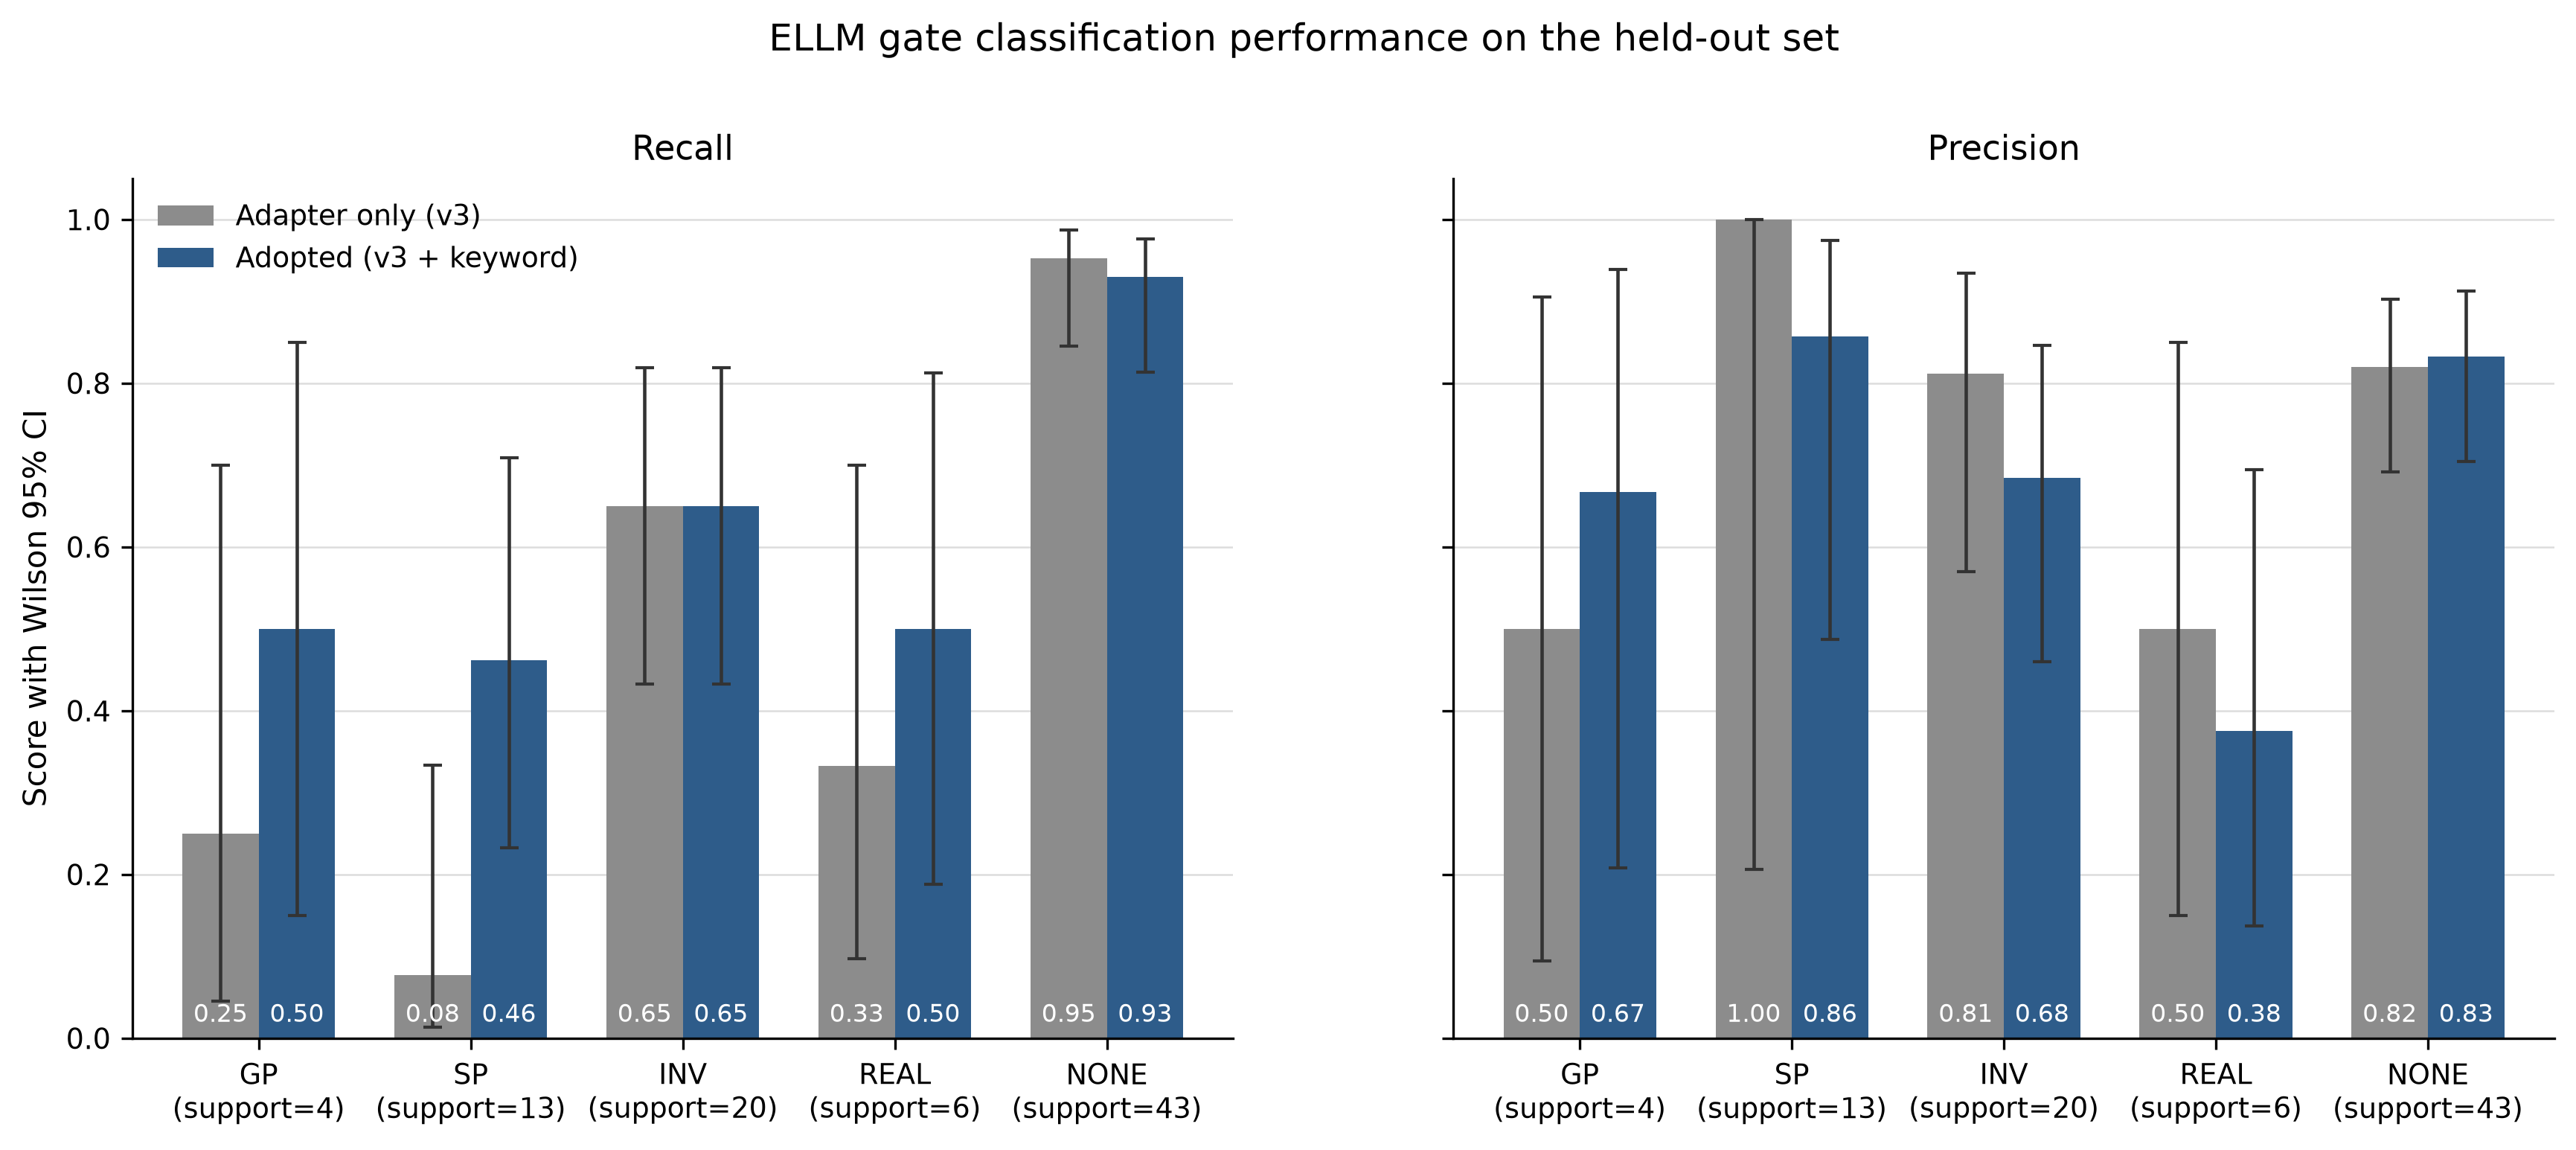
\includegraphics[width=0.85\linewidth]{Figures/G14_ellm_holdout.png}
\caption{Front-end classifier held-out recall and precision per category (Wilson 95\% CIs on recall). Adapter alone vs.\ adapter + keyword layer.}
\label{fig:ellm_holdout}
\Description{Bar chart of recall and precision per IPQ category on the held-out set.}
\end{figure}

Decomposing the two layers shows that the keyword layer buys recall at the cost of precision. Relative to the adapter alone, it raised recall for SP by $+.385$, GP by $+.250$, and REAL by $+.167$, left INV unchanged, and lowered NONE by $-.023$; precision fell for SP ($-.143$), INV ($-.128$), and REAL ($-.125$). A retrained adapter was evaluated against the deployed one and not adopted, as it lost SP recall ($-.077$) and produced a lower combined macro $F_1$ ($0.492$ vs.\ $0.567$).

Pipeline reach was measured on the 21 sessions for which the full audit was run (Figure~\ref{fig:reach_funnel}). Of the 294 item slots (14 items $\times$ 21 sessions), 289 received at least one candidate row. Of the 1{,}985 candidate rows that reached the scoring stage, 843 ($42.5\%$) were assigned a score, and 823 of those 843 passed the evidence gate into the primary indicator. Of the 92 item cells that remained empty, 87 were lost at the scoring stage; only 5 were lost at routing or at the evidence gate. A targeted keyword expansion recovered $12$ of $12$ missed INV utterances and $15$ of $19$ missed SP utterances.

\begin{figure}[t]
\centering
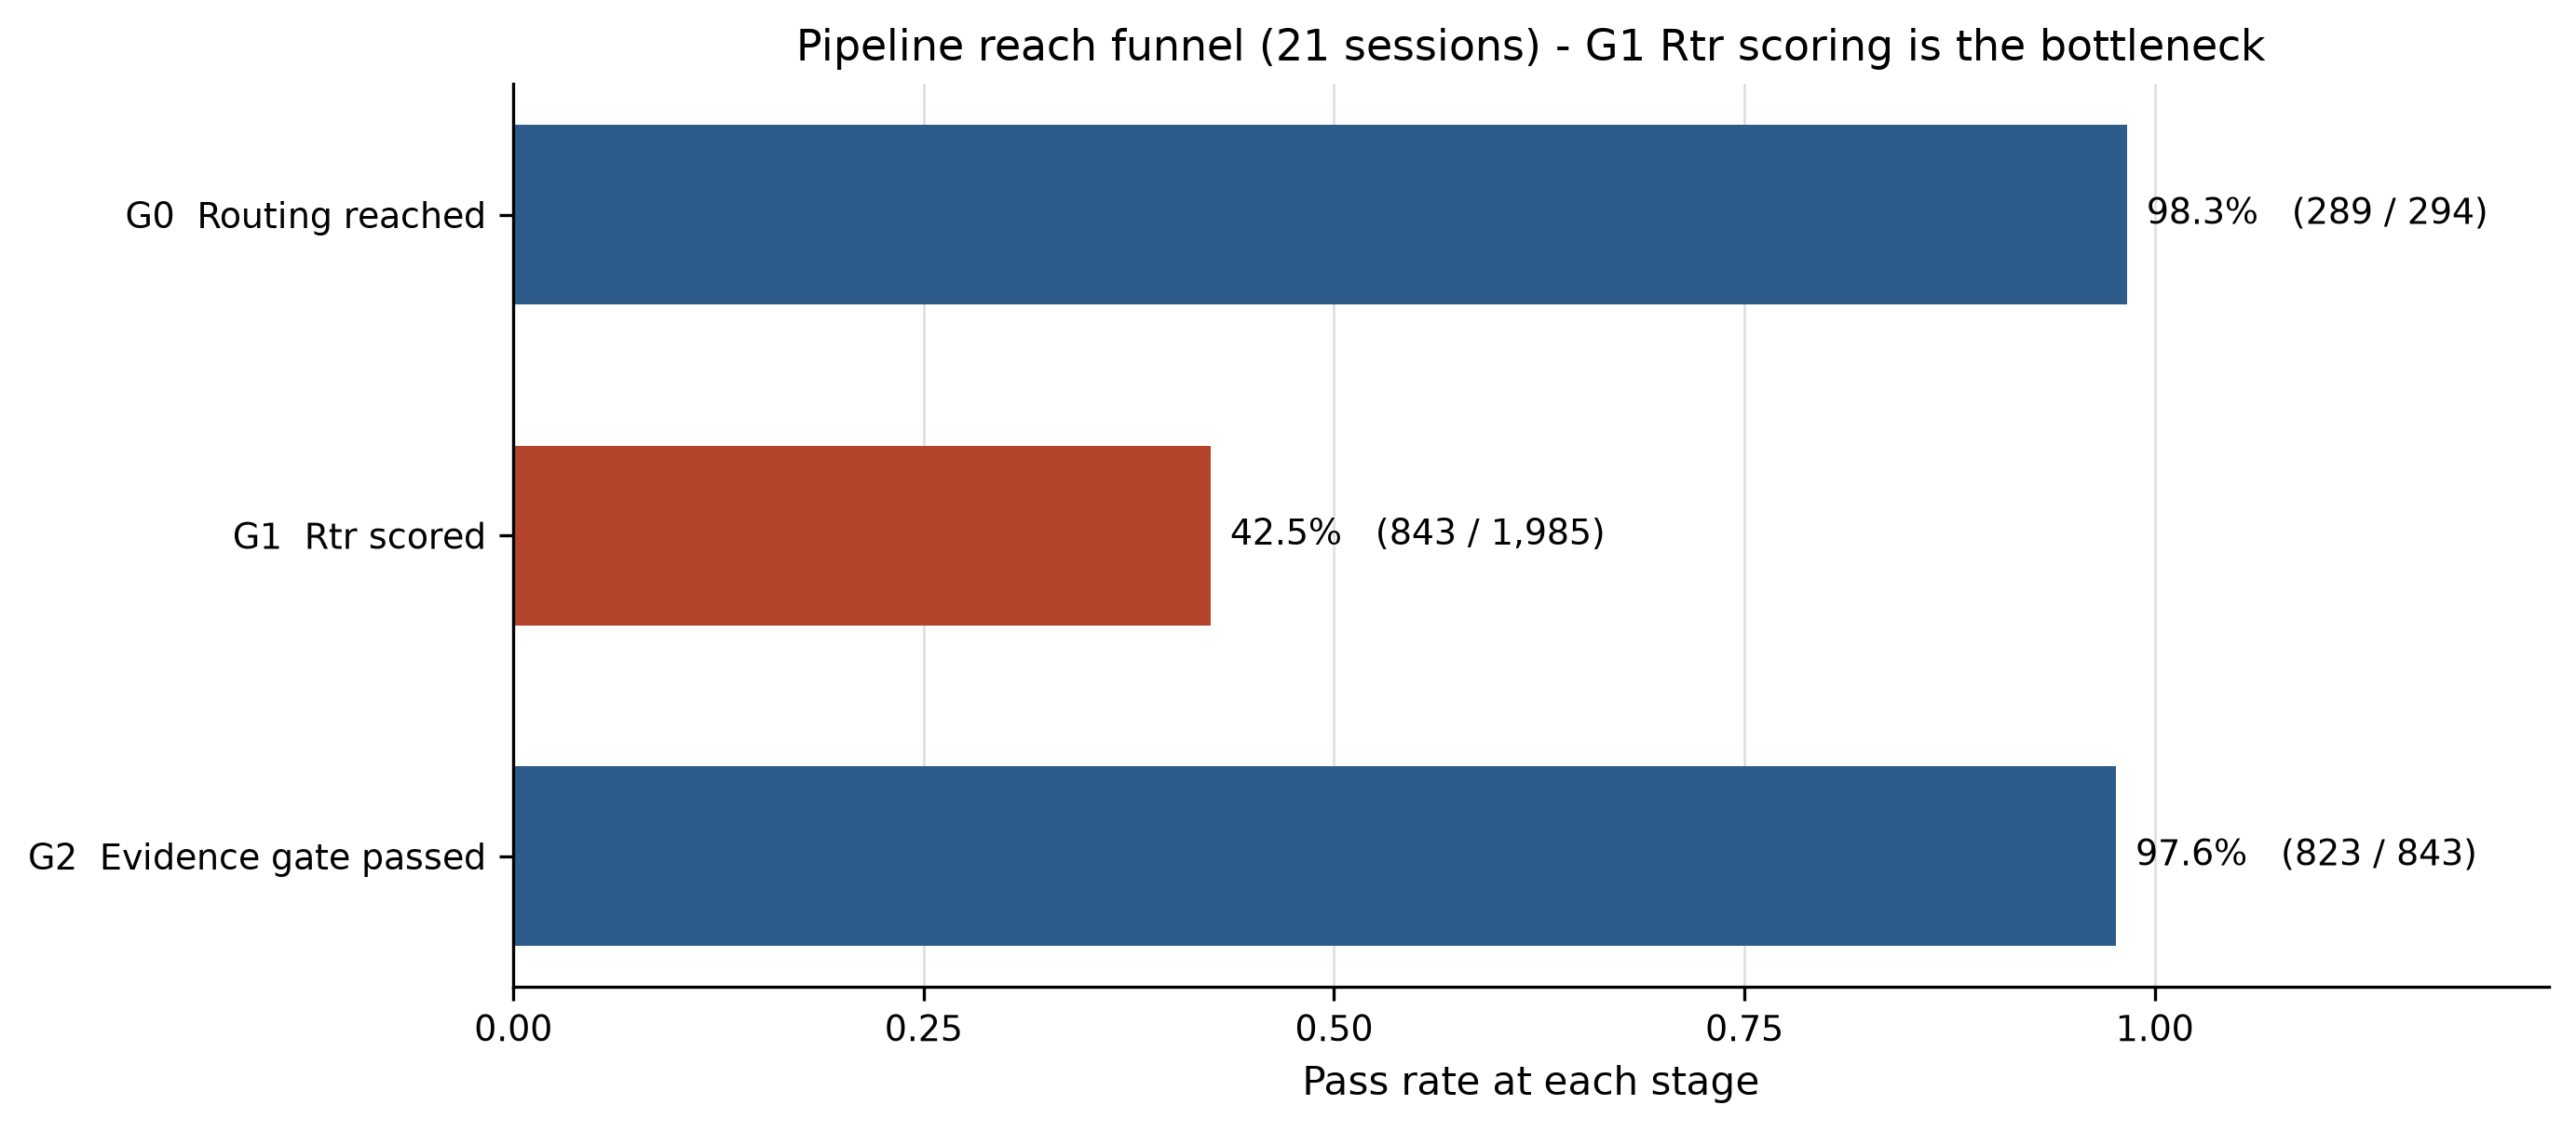
\includegraphics[width=0.85\linewidth]{Figures/G15_reach_funnel.png}
\caption{Pipeline reach funnel over the 21-session audit: candidate rows, scored items, and items that passed the evidence gate.}
\label{fig:reach_funnel}
\Description{Funnel chart from candidate rows through scored items to gate-passed items.}
\end{figure}


\subsection{Component Ablations and Negative Results}
\label{subsec:ablation}

Three components were evaluated in isolation during development and several alternatives were discarded; we report both because they locate where the pipeline's behavior comes from and where it does not.

\paragraph{Construct ontology and relation graph.}
Each of the 14 IPQ items is represented by a card (sub-indicators, boundary rules against neighboring items, and a guide paragraph), and the cards are linked by a relation graph of 62 typed edges, most of them routing edges that send a cue back to the item it belongs to. The drafter receives the cards, and the drafter and reviewer prompts receive a relation hint for the item under consideration. During development the ontology was tuned against a gold set of 65 utterances with known item assignments, using a retrieval harness as a coverage test; seven refinement steps raised gold recall from $.708$ to $1.000$. The harness is a development instrument, not the deployed routing (Section~\ref{subsec:rq2}), and the gold set is small (3--8 utterances per item), so this is a coverage check, not a precision estimate.

\paragraph{End-to-end ablation of the ontology on 12 sessions.}
A scoring-stage ablation was run on 12 sessions (four participants $\times$ three games, 894 utterances). The ablated condition emptied the item cards (names, keywords, guide text, learned examples) and removed all 62 relation edges while keeping the sub-indicator skeleton that generates the scoring cells; the deployed front-end output was reused upstream, so the comparison covers the scoring stage only. Two side effects are noted: the number of drafter calls was unchanged, and removing the guides disabled the improvement-path switch, so the ablated condition also differs by that routing change.

Session-level agreement with the questionnaire fell: the correlation with the total dropped from $r=.712$ to $.484$, mean absolute error rose from $0.517$ to $0.676$, and the within-participant top-1 match fell from 2 to 1 of the four participants (Table~\ref{tab:ablation_ontoC}).

The ablation also locates where the layer acts. Individual ratings were largely preserved: across the 442 cells scored under both conditions, $92.1\%$ of paired scores agreed within $0.5$ scale points ($48.6\%$ identical; mean signed difference $+0.03$). What moved was the assignment of evidence to items: of the 168 item slots, 123 carried evidence in the deployed condition and 109 under ablation, with SP falling from 51 to 28 and INV rising from 16 to 31. The subscale that lost the most slots is also the one whose correlation moved most (SP, $.053 \rightarrow -.320$), whereas REAL, which kept most of its slots, was unchanged ($.806 \rightarrow .798$). Because the session score is a mean over evidenced items, the layer's contribution on this evidence lies in evidence-to-item attribution, not in the severity of individual ratings.

The INV level offset was almost unchanged ($-0.742 \rightarrow -0.714$), consistent with the INV gap arising outside the rating of individual cells (Section~\ref{sec:discussion}). Four limits apply: the ablation is confined to the scoring stage; condition A is the deployed run, not a fresh replicate, so rater stochasticity is not separated from the gap; card content and relation edges were removed together, so their contributions cannot be credited separately; and with $n=12$ the values are descriptive, and GP and SP correlations were already near zero in the deployed condition, so their change of sign is not evidence that a working signal was lost.
\begin{table}[t]
\centering
\caption{End-to-end scoring-stage ablation of the construct ontology and relation graph on 12 sessions (four participants $\times$ three games; 894 utterances; 168 item slots). Condition A is the deployed run; condition C empties the card content and removes all 62 relation edges, retains the sub-indicator skeleton, and reuses the 1-Rvr output upstream. Correlations, errors, and level offsets are against the participant questionnaire; evidence slots count item slots carrying at least one piece of supporting evidence. The GP row is computed on the 11 sessions carrying GP evidence in both conditions; all other rows use 12. Cell-level agreement (442 paired cells) is reported in the text. Values are descriptive; no significance tests are reported at $n=12$.}
\label{tab:ablation_ontoC}
\small
\begin{tabular}{lrrr}
\hline
Measure & A & C & $\Delta$ \\
\hline
Session $r$ vs.\ questionnaire, total & $.712$ & $.484$ & $-.228$ \\
\quad GP & $.019$ & $-.502$ & $-.521$ \\
\quad SP & $.053$ & $-.320$ & $-.373$ \\
\quad INV & $.579$ & $.643$ & $+.064$ \\
\quad REAL & $.806$ & $.798$ & $-.008$ \\
Mean absolute error, total & $0.517$ & $0.676$ & $+0.159$ \\
Level offset, INV & $-0.742$ & $-0.714$ & $+0.028$ \\
Top-1 game match (of 4 participants) & $2$ & $1$ & $-1$ \\
Evidence slots, SP (of 60) & $51$ & $28$ & $-23$ \\
Evidence slots, INV (of 48) & $16$ & $31$ & $+15$ \\
Evidence slots, REAL (of 48) & $45$ & $39$ & $-6$ \\
Evidence slots, GP (of 12) & $11$ & $11$ & $0$ \\
\hline
\end{tabular}
\end{table}

\paragraph{Keyword layer in the front-end classifier.}
On the 73-utterance hold-out set, adding a keyword layer to the fine-tuned classifier raised SP recall from $.077$ to $.462$ at a precision cost from $1.000$ to $.857$ and GP recall from $.250$ to $.500$, while INV recall stayed at $.650$ (Figure~\ref{fig:ellm_holdout}); exact-set agreement was $.726$ for both variants. An error analysis of 31 missed utterances found the classifier accounting for most INV detections and the keyword layer for all SP detections, so the two layers cover different constructs.

\paragraph{What did not work.}
Interventions at the scoring stage repeatedly failed to improve agreement with the questionnaire. Injecting empirical anchors into the rater prompt worsened every metric on a paired check (quadratic-weighted $\kappa$ $.188\rightarrow.136$) and was reverted. Assigning maximal scores to exclamatory utterances left the INV4--questionnaire correlation unchanged ($.056\rightarrow.045$). Replacing mean with max aggregation halved the INV offset ($-1.144\rightarrow-0.500$) without recovering rank agreement ($r$ $.047\rightarrow.021$), and dropping the least-covered INV items widened the offset ($-0.554\rightarrow-0.641$ and $-0.710$). Projecting embeddings onto construct axes failed for the full item set because of synonym overlap among the realism items, and nearest-neighbor example injection had no measurable effect. These failures showed that the INV gap was not in the rater; the human-coder comparison later located it at the aggregation gate (Section~\ref{sec:discussion}).


\subsection{RQ3: Effect of the Think-Aloud Protocol on Reported Presence}
\label{subsec:rq3}

Table~\ref{tab:group} and Figure~\ref{fig:group_forest} contrast the two groups on the five IPQ measures. The TAP group reported higher presence on the IPQ total ($+0.441$, $t(26.2)=2.294$, $p=.030$, $d=0.81$), with the largest subscale difference on INV ($+0.656$, $t(30.0)=2.104$, $p=.044$, $d=0.74$). After Holm--Bonferroni correction across the five measures, none of the differences remained significant (IPQ total $p_{\mathrm{Holm}}=.150$; INV $p_{\mathrm{Holm}}=.176$). The effect size for the IPQ total was Hedges' $g=0.791$, 95\% CI $[0.086,\ 1.495]$, with a lower bound only marginally above zero. The think-aloud instruction did not raise workload: the TAP group's RTLX ($40.2$) did not differ detectably from the non-TAP group's ($35.1$; $p=.415$), and no individual TLX item differed either (Table~\ref{tab:workload}, all $p \geq .15$). Nor did it lower presence: the TAP group's IPQ total was higher, not lower, than the non-TAP group's.

\begin{table}[t]
\centering
\caption{Group comparison on participant-level means (Welch's $t$-test, $n=16$ per group). Asterisks mark uncorrected $p<.05$; no measure remains significant after Holm--Bonferroni correction across the five measures.}
\label{tab:group}
\small
\begin{tabular}{lccccccc}
\hline
Measure & TAP $M$ ($SD$) & non-TAP $M$ ($SD$) & Diff & $t$ & $p$ & $p_{\mathrm{Holm}}$ & $d$ \\
\hline
IPQ total & $4.202$ ($0.427$) & $3.762$ ($0.639$) & $+0.441$ & $2.294$ & $.030$* & $.150$ & $0.81$ \\
GP & $4.833$ ($0.621$) & $4.271$ ($1.097$) & $+0.562$ & $1.785$ & $.087$ & $.261$ & $0.63$ \\
SP & $4.471$ ($0.408$) & $4.229$ ($0.836$) & $+0.242$ & $1.039$ & $.310$ & $.310$ & $0.37$ \\
INV & $4.323$ ($0.883$) & $3.667$ ($0.881$) & $+0.656$ & $2.104$ & $.044$* & $.176$ & $0.74$ \\
REAL & $3.589$ ($0.583$) & $3.146$ ($0.821$) & $+0.443$ & $1.759$ & $.090$ & $.261$ & $0.62$ \\
\hline
\end{tabular}
\end{table}

\begin{table}[t]
\centering
\caption{Workload by group: NASA-TLX items and RTLX (0--100; participant-level means over the three games; Welch's $t$-test, $n=16$ per group). Asterisks mark uncorrected $p<.05$; $p_{\mathrm{Holm}}$ is corrected across the seven rows.}
\label{tab:workload}
\small
\begin{tabular}{lcccccc}
\hline
Measure & TAP $M$ ($SD$) & non-TAP $M$ ($SD$) & Diff & $t$ & $p$ & $p_{\mathrm{Holm}}$ \\
\hline
Mental demand & $34.6$ ($23.2$) & $28.1$ ($19.3$) & $+6.5$ & $.86$ & $.398$ & $1.000$ \\
Physical demand & $37.5$ ($24.8$) & $32.5$ ($22.6$) & $+5.0$ & $.60$ & $.555$ & $1.000$ \\
Temporal demand & $31.2$ ($22.9$) & $29.8$ ($21.8$) & $+1.5$ & $.18$ & $.855$ & $1.000$ \\
Performance & $52.5$ ($18.8$) & $43.8$ ($19.6$) & $+8.8$ & $1.29$ & $.208$ & $1.000$ \\
Effort & $58.5$ ($17.3$) & $48.8$ ($20.5$) & $+9.8$ & $1.46$ & $.155$ & $1.000$ \\
Frustration & $26.9$ ($21.3$) & $27.7$ ($22.8$) & $-0.8$ & $-0.11$ & $.916$ & $1.000$ \\
RTLX & $40.2$ ($16.6$) & $35.1$ ($18.3$) & $+5.1$ & $.83$ & $.415$ & $1.000$ \\
\hline
\end{tabular}
\end{table}

\begin{figure*}[t]
\centering
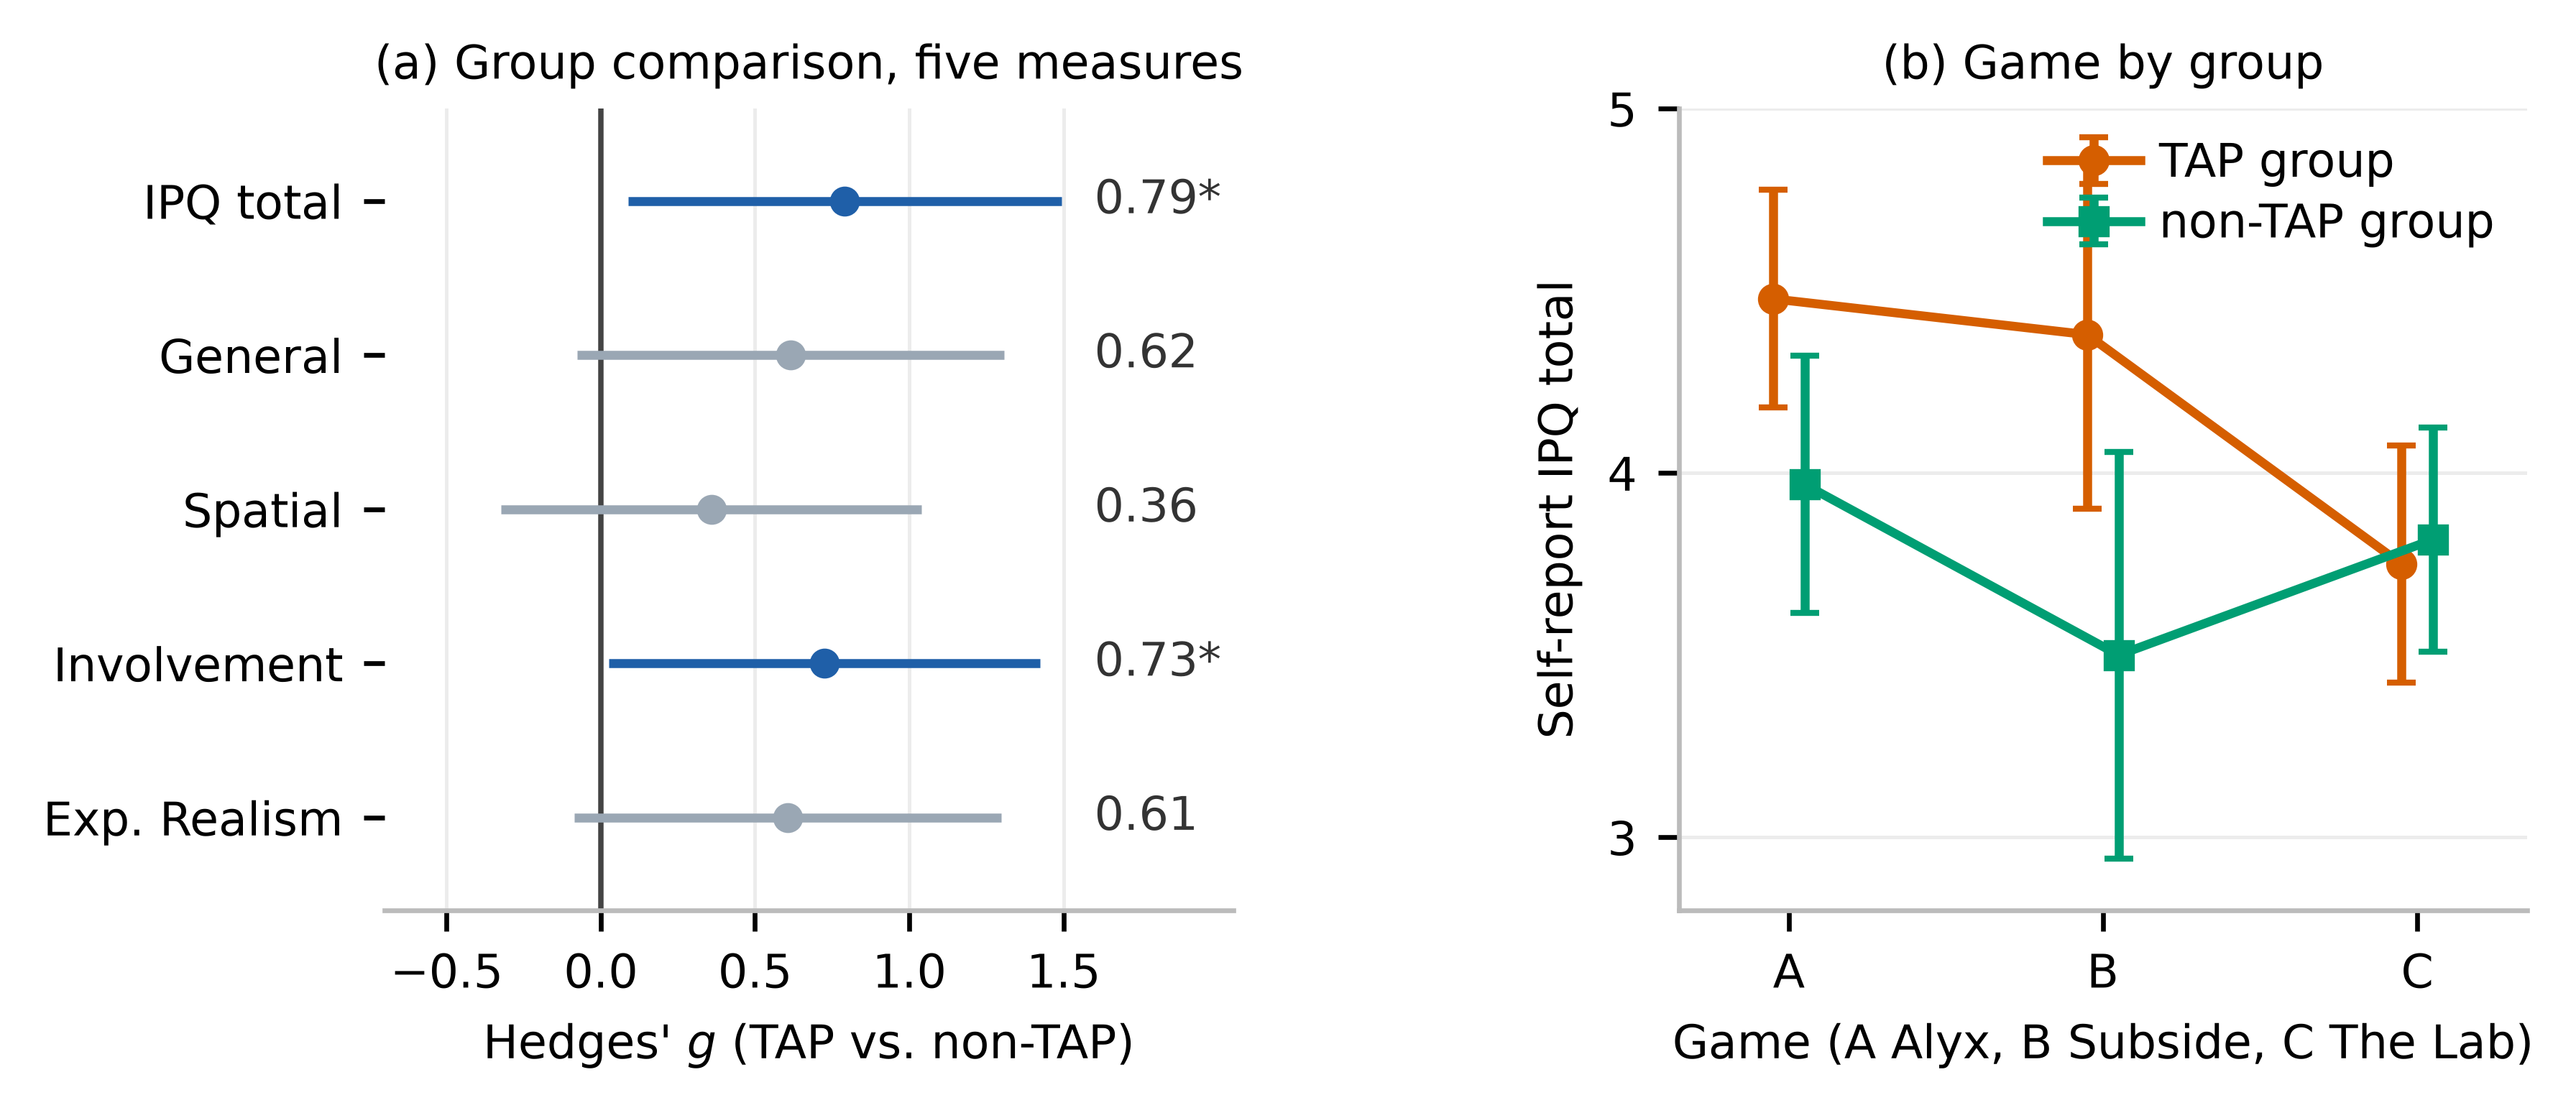
\includegraphics[width=0.76\textwidth]{Figures/F10_11_rq3_pair.png}
\caption{Group comparison on the five IPQ measures (a) and the game by group pattern on the self-reported IPQ total (b). 
In (a), each row is Hedges' $g$ with its 95\% confidence interval and the value at the right is that effect size; asterisks mark uncorrected $p<.05$, no measure remains significant after Holm--Bonferroni correction across the five measures, and both $p$ values are given in Table~\ref{tab:group}. In (b), points are group means with 95\% confidence intervals ($n=16$ per group).}
\Description{Two square panels side by side. The left panel is an interval plot of five standardized group differences with a zero reference line. The right panel plots self-reported IPQ totals for the two groups across the three VR games with confidence intervals.}
\label{fig:group_forest}
\end{figure*}

Two observations qualify the group difference. First, the TAP group scored higher on every measure, and on workload (Table~\ref{tab:workload}), so a general response-intensity difference cannot be separated from a presence-specific effect with these data. 
Second, the difference was not uniform across games (Figure~\ref{fig:group_forest}): at the session level it was present for Alyx ($+0.509$, $p=.026$) and Subside ($+0.879$, $p=.016$) but absent for The Lab ($-0.067$, $p=.753$).



Assignment and order were balanced. Stratification by motion-sickness susceptibility and prior VR experience was fully balanced across the two groups (4/4/4/4 per cell), with no group difference in susceptibility scores ($p=.822$) and no imbalance in game-order assignment ($\chi^2$ $p=.693$). A test for order effects across the three session positions was null ($p=.945$). Entering stratum, game order, and susceptibility as covariates in a participant-level regression left the coefficient essentially unchanged ($+0.440 \rightarrow +0.411$) while moving the $p$ value to the boundary ($.029 \rightarrow .052$) with 24 residual degrees of freedom.

Three data anomalies were identified from the session logs: one non-TAP participant ran the second game with passthrough enabled, one non-TAP participant completed the workload questionnaire from recall on the following day, and one non-TAP participant executed a game order different from the assigned one. Excluding the first two in a sensitivity analysis left the result unchanged ($+0.441 \rightarrow +0.422$, $p=.030$).

Independently of group, the three games differed in reported presence (Table~\ref{tab:game}). Alyx yielded the highest IPQ total and The Lab the lowest, with the Alyx--The Lab contrast the only reliable pairwise difference ($+0.440$, $t(31)=3.516$, $p=.001$). The game difference was carried by SP and REAL, on both of which Alyx exceeded The Lab ($p<.001$), whereas INV did not differ across games.

\begin{table}[t]
\centering
\caption{Self-reported IPQ total and subscales by game, both groups combined ($n=32$ participants; $M$ ($SD$) of participant-level scores), and paired contrasts within participants (mean difference and paired-$t$ $p$, $df=31$; $t$ values in the accompanying CSV). Asterisks mark uncorrected $p<.05$.}
\label{tab:game}
\small
\begin{tabular}{lccc cc cc cc}
\hline
 & \multicolumn{3}{c}{$M$ ($SD$)} & \multicolumn{2}{c}{Alyx $-$ Subside} & \multicolumn{2}{c}{Alyx $-$ The Lab} & \multicolumn{2}{c}{Subside $-$ The Lab} \\
Scale & Alyx & Subside & The Lab & Diff & $p$ & Diff & $p$ & Diff & $p$ \\
\hline
Total & $4.22$ ($0.66$) & $3.94$ ($1.06$) & $3.78$ ($0.59$) & $+0.283$ & $.122$ & $+0.440$ & $.001$* & $+0.156$ & $.415$ \\
GP & $4.84$ ($1.02$) & $4.38$ ($1.39$) & $4.44$ ($1.01$) & $+0.469$ & $.007$* & $+0.406$ & $.051$ & $-0.062$ & $.813$ \\
SP & $4.66$ ($0.61$) & $4.29$ ($1.09$) & $4.10$ ($0.79$) & $+0.362$ & $.041$* & $+0.556$ & $<.001$* & $+0.194$ & $.337$ \\
INV & $4.01$ ($1.27$) & $3.79$ ($1.23$) & $4.19$ ($1.03$) & $+0.219$ & $.350$ & $-0.180$ & $.387$ & $-0.398$ & $.099$ \\
REAL & $3.74$ ($0.85$) & $3.54$ ($1.28$) & $2.82$ ($1.14$) & $+0.203$ & $.441$ & $+0.922$ & $<.001$* & $+0.719$ & $.016$* \\
\hline
\end{tabular}
\end{table}


\section{DISCUSSION}
\label{sec:discussion}

\subsection{RQ1: What Speech-Derived Scores Capture Within the TAP Group}

Speech recovered the direction of presence but not its level. On participants never used to tune the pipeline, the speech-derived IPQ total tracked the self-reported total (Section~\ref{subsec:rq1_convergence}), and within each participant it usually identified which game had felt more present (Section~\ref{subsec:rq1_within}), supporting H2. It did not reproduce the survey's level: speech totals ran about a quarter of a point lower. That gap is real but smaller than the questionnaire's own measurement error, so at the group level the two totals are equivalent.

Why lower, when H3 predicted higher? We postulate that the offset comes from how the pipeline handles absence. Almost all of it sits in Involvement (Section~\ref{subsec:rq1_convergence}): two INV items ask whether the player was \emph{unaware} of the real world, and such absence rarely appears in speech as a statement. The evidence gate admits an item only when speech supports it, so these items stay unscored while the survey still rates them. Human coders did find INV evidence in most compared sessions (Section~\ref{subsec:rq1_reliability}), which shows the gap is a scoring rule, not silence. Consistent with this, calibrating INV removed most of the level offset without changing any direction indicator. Moment-to-moment speech therefore reports what is present; the retrospective survey also rates what was absent.

Three limits apply. The five cases in which the pipeline missed a participant's top game all involved the same pair of titles, so the errors are content-specific rather than random. Equivalence holds for group means, not individuals, and its margin was set after seeing the data. And the offset returned on the held-out participants after calibration had removed it on the development set: calibration transfers rank and variation, not absolute level.

\textbf{Within a participant, the speech-derived score says which session felt more present; it does not yet say how present in absolute terms.}

\subsection{RQ2: Speech Scores of the TAP Group Against the Non-TAP Survey}

\note{Pending: comparison of TAP speech-derived scores with non-TAP self-reported scores (analysis in progress).}

\subsection{RQ3: Did Thinking Aloud Itself Change Presence?}

H4 predicted lower presence and higher workload for the TAP group; we observed neither. The TAP group reported presence at least as high as the non-TAP group on every IPQ measure (Table~\ref{tab:group}), and no workload item differed between groups (Table~\ref{tab:workload}). After Holm correction across the five measures, no difference remained significant. We read this as a preliminary null against reactivity: in this sample, concurrent verbalization did not measurably degrade presence.

Why might the direction have reversed? With these data we cannot separate a presence effect from a general tendency of the TAP group to answer more intensely, since it scored higher on workload too. The pattern was also not uniform: it appeared for two games and was absent for The Lab, and the confidence interval on the total barely excludes zero. One further observation needs a larger study: the spatial-presence items were far less internally consistent in the TAP group than in the non-TAP group while the means matched (Section~\ref{subsec:sample}). If it replicates, verbalizing may perturb self-report not by shifting the mean but by loosening the coherence of the answers.

\textbf{Thinking aloud did not cost presence: it added no measurable workload, and the TAP group reported presence at least as high as the group that played without the instruction.}

\subsection{What the System Contributed (H1)}

The local front end sorted utterances into the four IPQ constructs well enough to feed the scoring chain: nearly every item slot received candidate evidence and nearly every scored item passed the evidence gate, with the losses at the scoring stage rather than at routing (Section~\ref{subsec:rq2}). Its INV recall was mid-range, so the INV gap above is not a routing failure. H1 is supported in the sense that speech can be quantified onto IPQ subscales, with the coverage limits documented above.

\textbf{The on-device front end is not the bottleneck; the evidence gate is where coverage is decided.}

\subsection{Implications for VR Evaluation Practice}

Speech-derived scoring can complement the post-session survey when the question is a within-person comparison across content and no questionnaire can be given between sessions. It should not yet be used as an absolute presence score against an external reference. And a session's score is a statement about the items the player's speech supported: an uncovered item should stay missing rather than be imputed as zero.

\paragraph{Cost.}
Hand-coding the 3{,}595 TAP utterances against 14 items would take 60--180\,s per utterance, a bracket derived from timed deductive coding~\cite{chew2023llm}; with two coders and 10\% adjudication, as verbal-protocol analysis conventionally requires~\cite{chi1997quantifying}, that is roughly 132--396 person-hours before transcription. The pipeline's recorded API cost for scoring was USD 0.98--2.22 per session, about USD 50--110 for all 48 sessions. These are operating costs only; development iterations are excluded, and the quality of manual coding was not measured. Every intermediate judgment is logged, which makes the automated path auditable in a way manual coding notes rarely are.

\section{LIMITATIONS AND FUTURE WORK}
\label{sec:limitations}

Several limitations should be considered when interpreting the present findings.
First, the TAP analyses were based on 16 participants across 48 sessions, with an even smaller held-out confirmation sample. Although the results showed promising correspondence between LLM-derived and self-reported IPQ scores, larger and fully independent samples are needed to establish the generalizability of the proposed approach across participants and VR content.

In addition, verbal evidence was uneven across IPQ items, particularly for Involvement (INV). Because the current system calculates scores only from items supported by sufficient think-aloud evidence, the resulting scores are not always based on all 14 IPQ items. Future work will refine the evidence and aggregation rules and investigate complementary multimodal signals, such as gaze, head and hand movements, and gameplay events, to improve item coverage without requiring additional verbalization.

Another limitation is that the multi-agent scoring chain currently relies on commercial LLM APIs, which introduces concerns regarding privacy, reproducibility, and scalability. Future work will therefore explore locally deployable or open-weight models for the Drafter, Reviewer, and Rater roles.

The current findings also primarily support relative comparisons across VR experiences rather than absolute presence estimation. The observed score offset and exploratory equivalence margin limit direct interchangeability with conventional IPQ scores. Future studies should validate predefined equivalence bounds and further calibrate LLM-derived scores using larger independent datasets.

Finally, the influence of TAP itself remains inconclusive because the TAP and non-TAP comparison was between participants and involved a relatively small sample. Future work should use larger samples and counterbalanced within-participant designs, with equivalent VR familiarization across conditions, to more clearly isolate the effect of concurrent verbalization on presence and workload.

% Several limitations qualify the scope of the current findings.
% First, the sample size for the speech-derived analyses is $16$ participants ($48$ sessions), which is adequate for the within-person direction indicators reported here (permutation $p<.005$ on top-1 and on pairwise direction) but leaves the complete-rank indicator underpowered ($31\%$ vs.\ $17\%$, $p=.11$) and yields wide confidence intervals on the participant-level correlations. The held-out confirmation sample is smaller still (nine participants, $27$ sessions); its correlation is significant but imprecisely estimated (clustered $95\%$ CI $[+.26, +.85]$), and the pipeline was developed on the same population, so replication on an independent sample remains necessary. A larger TAP sample would tighten these estimates and also allow subgroup analyses that the current data do not support.

% Third, the multi-agent scoring chain uses commercial LLM API models as the drafter, reviewer, and rater. This limits data privacy, ties reproducibility to versioned commercial models, and makes cost a scaling constraint for larger studies.

% Fourth, INV items are the least covered by speech in this sample, and the within-participant INV correlation is null. The human-coder comparison attributes much of this gap to the aggregation rule for absence-scored items, not to silence (Section~\ref{sec:discussion}), so INV coverage should improve if that rule is relaxed, but the comparison rests on 12 sessions and two coders.

% Fifth, speech-derived totals sit below survey totals by about a quarter of a point on the $0$--$6$ scale, and the INV-side calibration term is a first pass that removes the level offset on INV but does not correct the absolute-value gap in general. The pipeline currently compares sessions within a participant; it does not yet produce absolute presence scores against an external reference.

% Sixth, the RQ3 group comparison is between participants and, at $n=16$ per group, is not powered to detect small effects; the uniform elevation of the TAP group on non-presence measures (workload, cybersickness) means that a general response-intensity difference cannot be separated from a presence-specific effect with the current design.

% Finally, the equivalence margin was derived by us: no published margin exists for presence questionnaires, and prior VR equivalence studies likewise set their own bounds~\cite{lee2012equivalence,sanaei2024scene}. Our margin is anchored to the questionnaire's measurement error, and equivalence held under every rule that uses the full-sample $SD$, but it was specified after the data were collected, so the equivalence analysis is exploratory. Equivalence was also established for group-level means only: the limits of agreement and the concordance correlation show that the two measures are not interchangeable for an individual participant.



% Three directions follow directly from the limitations above. First, the INV gap has been traced to the aggregation rule for absence-scored items (Section~\ref{sec:discussion}); the next step is to revise that rule and re-score the existing sessions, and only then to decide whether new content or new operationalizations of INV1 and INV3 are needed.

% Second, augmenting speech with a stream that participants do not have to verbalize, for example, gameplay events, head- and hand-pose signals, or gaze, would allow the scoring chain to route around the INV gap and provide a converging channel for the total score. This addresses the coverage limitation without asking participants to say more.

% Third, a within-participant design in which the same participant plays with and without the think-aloud instruction on the same VR content, and a scaled-up between-participants sample, would tighten the RQ3 conclusion beyond the current preliminary null.

% \section{CONCLUSION}
% \label{sec:conclusion}

% This paper asked whether concurrent think-aloud speech, scored by an evidence-gated multi-agent LLM pipeline, can stand in for self-reported presence. The answer is a qualified yes. On participants held out from pipeline selection, the speech-derived IPQ total converged with the survey, and within a participant it reliably told which of three VR games had felt more present, while sitting systematically lower in absolute level. Where the two measures part ways, the reason is now largely known: involvement items are scored from the absence of speech signals, and the evidence gate drops them at aggregation, so the gap lies in a scoring rule, not in what participants say or in how the rater judges it. Human coders agreed with the pipeline about as well as they agreed with each other. Thinking aloud did not measurably lower reported presence. The practical claim is narrow but useful: for the purpose the IPQ serves in comparative VR evaluation, telling which session felt more present to the same player, an evidence-gated speech score can fill that role alongside post-session self-report.


% The LLM-derived scores showed meaningful correspondence with self-reported IPQ scores and captured relative differences in presence across VR experiences, particularly within the same participant, although systematic score offsets and uneven evidence coverage, especially for Involvement, currently limit their use as interchangeable absolute IPQ scores. 


\section{CONCLUSION}
\label{sec:conclusion}

Creating a convincing sense of ``being there'' is central to the user experience of VR, making presence an important criterion for evaluating immersive systems and content. 
This work introduced an evidence-gated LLM-based system for converting think-aloud utterances into IPQ-based presence scores and evaluated its use as a complementary presence measure.
The LLM-derived scores showed meaningful correspondence with self-reported IPQ scores and captured relative differences in presence across VR experience.
% , particularly within participants. 
However, systematic score offsets and uneven coverage of subjective presence dimensions, especially the IPQ Involvement (INV) dimension, currently limit their use as interchangeable absolute IPQ scores.
The locally fine-tuned routing classifier successfully directed presence-related utterances to the downstream multi-agent scoring chain, enabling unstructured think-aloud data to be organized into IPQ-related evidence for quantitative scoring. Moreover, concurrent think-aloud showed no clear evidence of reducing experienced presence or substantially increasing workload in the present study. 
These findings support think-aloud-derived presence scores as a complementary measure for comparing VR experiences.
Future work should validate the approach with larger independent samples, improve evidence coverage and score aggregation, incorporate complementary behavioral signals, and further examine the influence of TAP on the VR experience.


% Future work should validate the approach with larger independent samples, improve evidence coverage and score aggregation, incorporate complementary behavioral signals, and further examine the influence of TAP using counterbalanced within-participant designs.


% The locally fine-tuned routing classifier also provided sufficient coverage for the downstream multi-agent scoring process, supporting the feasibility of transforming unstructured think-aloud utterances into structured presence estimates. 
% Moreover, concurrent think-aloud showed no clear evidence of reducing presence or substantially increasing workload in the present study. 
% These findings support think-aloud--derived presence scores as a complementary approach for comparative VR evaluation, while future work should validate the method with larger independent samples, refine evidence and aggregation rules, incorporate complementary behavioral signals, and further examine TAP reactivity using stronger within-participant designs.



\begin{acks}
This work was supported by 
the MSIT of Korea/IITP-ITRC under Grant IITP-2022-RS-2022-00156354; and 
National Research Foundation under Grant RS-2025-00514411.
The authors used AI tools for grammatical checking and linguistic refinement of the text, and Gemini 3.1 Pro image generation to draft the illustration of Figure~\ref{fig:teaser} and the layout of the pipeline example figure, which the authors then finished and labeled in Adobe Illustrator; all data shown are the authors' own.
\end{acks}


\bibliographystyle{ACM-Reference-Format}
\bibliography{references}
\clearpage
\appendix
\section{Supplementary Tables}
\label{sec:appendix}

Table~\ref{tab:within_by_construct} reports the same within-person indicators broken down by IPQ subscale (Section~\ref{subsec:rq1_within}).

\begin{table}[htbp]
\centering
\caption{Within-participant agreement by IPQ subscale. Participants missing any of their three games' speech-derived score on a subscale are excluded from that row (so $n<16$ for GP, SP, INV, REAL).}
\label{tab:within_by_construct}
\small
\begin{tabular}{lcccc}
\hline
Scale & $n$ & Complete rank & Top-1 & Pairwise \\
\hline
Total & 16 & $31\%$ & $69\%$ & $76\%$ \\
GP & 10 & $20\%$ & $50\%$ & $65\%$ \\
SP & 15 & $13\%$ & $40\%$ & $64\%$ \\
INV & 15 & $13\%$ & $73\%$ & $61\%$ \\
REAL & 16 & $19\%$ & $44\%$ & $59\%$ \\
\hline
\end{tabular}
\end{table}

Table~\ref{tab:convergence} reports convergence between the speech-derived and self-reported IPQ scores by aggregation level and scale on the pooled sample (Section~\ref{subsec:rq1_convergence}).

\begin{table}[htbp]
\centering
\caption{Convergence between speech-derived and self-reported IPQ scores, by aggregation level. Session level includes repeated measures within participants and should be read as an upper-bound estimate. Asterisks mark uncorrected $p<.05$.}
\label{tab:convergence}
\small
\begin{tabular}{llccc}
\hline
Level & Scale & $n$ & Pearson $r$ & $p$ \\
\hline
Session & Total & 48 & $+.419$ & $.003$* \\
Session & GP & 39 & $+.364$ & $.023$* \\
Session & SP & 47 & $+.251$ & $.089$ \\
Session & INV & 47 & $+.127$ & $.397$ \\
Session & REAL & 48 & $+.437$ & $.002$* \\
\hline
Participant & Total & 16 & $+.488$ & $.055$ \\
Participant & GP & 15 & $+.099$ & $.727$ \\
Participant & SP & 16 & $+.150$ & $.580$ \\
Participant & INV & 16 & $+.382$ & $.145$ \\
Participant & REAL & 16 & $+.518$ & $.040$* \\
\hline
Within-participant & Total & 48 & $+.386$ & $.007$* \\
Within-participant & GP & 38 & $+.416$ & $.009$* \\
Within-participant & SP & 47 & $+.293$ & $.046$* \\
Within-participant & INV & 47 & $-.055$ & $.715$ \\
Within-participant & REAL & 48 & $+.418$ & $.003$* \\
\hline
\end{tabular}
\end{table}

Table~\ref{tab:equivalence} lists all margin combinations tested for the participant-level equivalence analysis (Section~\ref{subsec:rq1_convergence}).

\begin{table}[htbp]
\centering
\caption{Equivalence of the speech-derived and self-reported IPQ totals at the participant level ($n=16$; observed offset $-0.232$, $SE=0.095$) under alternative margin definitions. $SEM = SD\sqrt{1-\alpha}$; $SDC = 1.96\sqrt{2}\,SEM$. The first row is the pre-declared primary rule.}
\label{tab:equivalence}
\small
\begin{tabular}{llccccl}
\hline
$\alpha$ source & $SD$ sample & $SEM$ & Rule & Margin & TOST $p$ & Verdict \\
\hline
Literature ($.87$)~\cite{schwind2019presence} & All 32 ($0.579$) & $0.209$ & SDC & $\pm0.579$ & $.001$ & equivalent \\
Literature ($.87$) & All 32 ($0.579$) & $0.209$ & $1.96\,SEM$ & $\pm0.409$ & $.041$ & equivalent \\
Own sample ($.816$) & All 32 ($0.579$) & $0.248$ & SDC & $\pm0.688$ & $<.001$ & equivalent \\
Own sample ($.816$) & All 32 ($0.579$) & $0.248$ & $1.96\,SEM$ & $\pm0.486$ & $.009$ & equivalent \\
Literature ($.87$) & PT only ($0.427$) & $0.154$ & SDC & $\pm0.426$ & $.029$ & equivalent \\
Literature ($.87$) & PT only ($0.427$) & $0.154$ & $1.96\,SEM$ & $\pm0.302$ & $.237$ & not established \\
\hline
\end{tabular}
\end{table}

Table~\ref{tab:calibration_prepost} lists all pre- and post-calibration values on the total and on the INV subscale (Section~\ref{subsec:rq1_convergence}).

\begin{table}[htbp]
\centering
\caption{Effect of the INV-side calibration ($+0.5535$) on level and on within-person direction indicators. Pre- and post-calibration values are reported side by side (calibration input file, $n=15$ participants with three fully covered games; the direction analyses in Section~\ref{subsec:rq1_within} use the $n=16$ sample without calibration).}
\label{tab:calibration_prepost}
\small
\begin{tabular}{llcc}
\hline
Scale & Indicator & Pre & Post \\
\hline
Total & Mean speech$-$survey level offset & $-0.221$ & $-0.134$ \\
Total & Mean absolute error & $0.603$ & $0.584$ \\
Total & Fraction $|error|\le 0.5$ & $45\%$ & $49\%$ \\
Total & Fraction speech $<$ survey & $64\%$ & $60\%$ \\
Total & Within-person top-1 (n=15) & $67\%$ & $60\%$ \\
Total & Within-person pairwise (n=15) & $77\%$ & $72\%$ \\
Total & Within-person complete rank (n=15) & $33\%$ & $33\%$ \\
INV & Mean speech$-$survey level offset & $-0.554$ & $-0.000$ \\
INV & Mean absolute error & $1.070$ & $0.845$ \\
INV & Fraction $|error|\le 0.5$ & $26\%$ & $45\%$ \\
INV & Within-person top-1 (n=15) & $73\%$ & $73\%$ \\
INV & Within-person pairwise (n=15) & $61\%$ & $61\%$ \\
INV & Within-person complete rank (n=15) & $13\%$ & $13\%$ \\
Side effect & Sessions crossing the $6.0$ ceiling & $0$ & $1$ \\
\hline
\end{tabular}
\end{table}
% ===== 부록 IPQ 14문항 표 (MCd 2026-09-11) — 07_appendix.tex 맨 끝 (\end{table} 마지막 줄 다음) 에 붙여넣기. 컨테이너 pdflatex 로 컴파일 확인 완료 (tabularx·array 는 main.tex 34행에서 이미 로드됨) =====

Table~\ref{tab:ipq_items} lists the 14 IPQ items~\cite{schubert2001experience} as administered in this study, with their subscale assignment, the anchors of the 0--6 response scale, and the three reverse-keyed items (SP2, INV3, REAL1); INV1 uses a reversed anchor by design and is not reverse-keyed~\cite{tran2024ipq}.

\begin{table}[htbp]
\centering
\caption{The 14 items of the Igroup Presence Questionnaire (IPQ) used in this study. Subscales: General Presence (GP), Spatial Presence (SP), Involvement (INV), Experienced Realism (REAL). Anchors are the labels of the 0 and 6 endpoints of the 0--6 scale. R marks the reverse-keyed items, whose scores were reversed ($6-\text{raw}$) before aggregation.}
\label{tab:ipq_items}
\small
\begin{tabularx}{\textwidth}{llX>{\raggedright\arraybackslash}p{3.4cm}c}
\hline
Item & Subscale & Wording & Anchors (0 / 6) & R \\
\hline
GP1 & GP & In the computer generated world, I had a sense of ``being there.'' & not at all / very much & \\
SP1 & SP & Somehow I felt that the virtual world surrounded me. & fully disagree / fully agree & \\
SP2 & SP & I felt like I was just perceiving pictures. & fully disagree / fully agree & R \\
SP3 & SP & I did not feel present in the virtual space. & did not feel / felt present & \\
SP4 & SP & I had a sense of acting in the virtual space, rather than operating something from outside. & fully disagree / fully agree & \\
SP5 & SP & I felt present in the virtual space. & fully disagree / fully agree & \\
INV1 & INV & How aware were you of the real world surrounding while navigating in the virtual world? (i.e., sounds, room temperature, other people, etc.) & extremely aware / not aware at all & \\
INV2 & INV & I was not aware of my real environment. & fully disagree / fully agree & \\
INV3 & INV & I still paid attention to the real environment. & fully disagree / fully agree & R \\
INV4 & INV & I was completely captivated by the virtual world. & fully disagree / fully agree & \\
REAL1 & REAL & How real did the virtual world seem to you? & completely real / not real at all & R \\
REAL2 & REAL & How much did your experience in the virtual environment seem consistent with your real world experience? & not consistent / very consistent & \\
REAL3 & REAL & How real did the virtual world seem to you? & about as real as an imagined world / indistinguishable from the real world & \\
REAL4 & REAL & The virtual world seemed more realistic than the real world. & fully disagree / fully agree & \\
\hline
\end{tabularx}
\end{table}


\end{document}